\documentclass[11pt,a4paper]{article}
\usepackage[T1]{fontenc}\usepackage[utf8]{inputenc}\usepackage{lmodern}
\usepackage{microtype}\usepackage{geometry}\geometry{margin=1in}
\usepackage{amsmath,amssymb,amsfonts,amsthm,mathtools}
\usepackage{graphicx,float,booktabs,array,multirow,enumitem,tabularx}
\usepackage[numbers,sort&compress]{natbib}
\usepackage[colorlinks=true,linkcolor=blue,citecolor=blue,urlcolor=blue]{hyperref}
\usepackage{caption,xcolor,siunitx,listings}
\emergencystretch=2em

\lstset{basicstyle=\ttfamily\small,breaklines=true,frame=single,
        columns=fullflexible,backgroundcolor=\color{gray!6}}

\newtheorem{theorem}{Theorem}\newtheorem{lemma}{Lemma}
\newtheorem{corollary}{Corollary}\newtheorem{proposition}{Proposition}
\newtheorem{definition}{Definition}\newtheorem{assumption}{Assumption}
\newtheorem{remark}{Remark}

\DeclareMathOperator{\Tr}{Tr}\DeclareMathOperator{\rank}{rank}
\newcommand{\cD}{\mathcal{D}}\newcommand{\cH}{\mathcal{H}}
\newcommand{\cN}{\mathcal{N}}\newcommand{\cR}{\mathcal{R}}
\newcommand{\cU}{\mathcal{U}}
\newcommand{\cC}{\mathcal{C}}
\newcommand{\norm}[1]{\left\lVert #1\right\rVert}
\newcommand{\ket}[1]{\lvert #1\rangle}
\newcommand{\proj}[1]{\lvert #1\rangle\!\langle #1\rvert}

\title{Adversarial Channel Equilibria for qLDPC Memories:\\
Bounded-Weight Fidelity Guarantees and\\
Reproducible Three-Code Bivariate-Bicycle Benchmarks}

\author{Saleh H.\ AlDaajeh$^{1}$, [AUTHOR 2: name]$^{2}$, [AUTHOR 3: name]$^{3}$\\[2pt]
[AUTHOR 4: name]$^{4}$, [AUTHOR 5: name]$^{5}$\\[4pt]
\small $^{1}$Independent Researcher, Information Systems and Security; \texttt{S.aldaajeh@gmail.com}\\
\small ORCID: \href{https://orcid.org/0000-0001-7810-9290}{0000-0001-7810-9290}\\
\small $^{2}$[AUTHOR 2: affiliation, email]\\
\small $^{3}$[AUTHOR 3: affiliation, email]\\
\small $^{4}$[AUTHOR 4: affiliation, email]\\
\small $^{5}$[AUTHOR 5: affiliation, email]\\[4pt]
\small Archive: prepared for Zenodo deposition; doi:10.5281/zenodo.20588043 (published June 2026)\\[2pt]
\small QEC Emulator v1.2.4~\cite{AlDaajeh2026emulator}
(ldpc~2.4.1, pymatching~2.4.0, numpy~2.4.4)}
\date{\today}

\begin{document}
\maketitle

%%-----------------------------------------------------------
\begin{abstract}
%%-----------------------------------------------------------
We formulate adversarial channel equilibrium (ACE) for qLDPC memories
as an \emph{injection-budget} game between a bounded-weight adversary
and a composed recovery, yielding an operational, device-measurable
value, with quantitative predictions subjected to a pre-registered
hardware test. The theory layer pairs two acknowledged tools---a channel-game minimax
saddle point and a Knill--Laflamme fidelity floor---with new elements: a spacetime-budget
correctability theorem with an explicit sharpness construction and a
device-aware composition bound, extended to CSS memories
(Theorem~\ref{thm:spacetime},
Corollaries~\ref{cor:css}--\ref{cor:stoch}), and a Pauli-channel bridge
converting measured logical failure rates into diamond-norm bounds
(Proposition~\ref{prop:bridge}). All experiments use the open-source
QEC Emulator v1.2.4 with deterministic seeds and SHA-256 provenance.
Across three bivariate-bicycle codes: an exhaustive BB[[72,12,6]]
certificate ($d=6$ exactly);
benchmarks in which BP+OSD lies far below two graphified
matching baselines (risk ratios $67.8\times$ to $>$183{,}000$\times$); a
pinned seven-decoder paired grid on 70{,}000 bit-identical instances (BP
augmentation closes the gap to BP+OSD; bare symmetry matching is
non-viable);
circuit-level corroboration inverting the BP+OSD/Relay-BP ordering; a
five-decoder re-analysis of the released Kunlun $[[18,4,4]]$
detector model; and hardware noise-model ablations. On
ibm\_marrakesh, calibration-informed placement lowered logical error in
all four configurations ($p=0.042$); a pre-registered
injection test confirmed the distance cliff, falsified the
independence-form stochastic bound at $p=0.10$, and found the
device-aware bound satisfied on every arm, replicating across cycles,
devices, and distance~7. The evidence assembles into a five-level
quantum memory integrity certification hierarchy (QMAL-1--5), with
syndrome-only monitoring proved insufficient.

\end{abstract}

\noindent\textbf{Keywords:} qLDPC; bivariate-bicycle codes; adversarial
channels; minimax; entanglement fidelity; BP+OSD; MWPM; DEM decomposition;
reproducible benchmarks; open-source scientific software.

%%-----------------------------------------------------------
\section{Introduction}
%%-----------------------------------------------------------

Fault-tolerant quantum computing and post-quantum cryptography are
strategically coupled~\cite{Shor1997,NISTFIPS203,NISTFIPS204,NISTFIPS205}.
The bivariate-bicycle (BB) code family~\cite{Bravyi2024} provides a
high-rate, weight-six qLDPC substrate suitable for both defensive
deployment and adversarial analysis.

\paragraph{Specific gap.}
Prior BB benchmarks~\cite{Bravyi2024,ShawRengaswamy2026} use BP+OSD;
this paper adds a transparent graphified DEM-MWPM reference baseline compatible with PyMatching-style graphlike inputs, together with a three-code same-protocol reproducibility archive with SHA-256 manifests.
We fill these gaps for the tested implementations and find that the two graphified baselines perform substantially worse than BP+OSD under this protocol.

\subsection{What this paper claims (precise)}

\begin{enumerate}[leftmargin=1.6em,label=(\roman*)]
  \item Minimax saddle point via Sion's theorem (acknowledged standard).
  \item Fidelity floor $+$ i.i.d.\ stochastic lower bound via Knill--Laflamme.
  \item Architectural scaling lemma on logical-operator weight.
  \item QEC Emulator v1.2.4 --- open-source software infrastructure for all
    experiments, with five independently extensible layers and SHA-256 provenance.
  \item BB72 certificate: $d=6$ exact, $t=2$ exhaustive, SHA-256 matrix pins.
  \item Three-code single-round BP+OSD vs DEM-MWPM, 10{,}000 trials, CIs,
    with a $10^{6}$-trial rare-event refinement at $p\in\{0.002,0.004\}$.
  \item Three-code repeated-cycle BP+OSD ($d$~rounds), 2{,}000--500 trials, CIs,
    plus 4{,}000--20{,}000-trial adaptive extensions.
  \item Three-code finite-size evidence (sub-threshold ordering, not formal FSS).
  \item Hardware ablation (simulation models only): SWAP routing, measurement noise, and gate-decoherence parameters materially affect the simulated CZ/MS gap; no real-hardware causal claim is made.
  \item UF-BFS provides a second graphified baseline; it also underperforms BP+OSD under the submitted protocol.
  \item Decoder-dependent ACE gap (Remark~\ref{rem:decoder-gap}; upgraded from
    proxy to bound under the Pauli approximation by
    Proposition~\ref{prop:bridge}).
  \item Injection-budget game: operational ACE value
    (Definition~\ref{def:acevalue}), spacetime-budget correctability theorem
    with sharpness construction (Theorem~\ref{thm:spacetime}), device-aware
    composition bound (Corollary~\ref{cor:stoch}).
  \item Pre-registered device test of the theory layer on ibm\_marrakesh
    (Appendix~\ref{app:injection}, 312 arms, 180{,}000 shots): weight-$t$
    worst-case injections bounded, weight-$(t{+}1)$ collapse at
    $92$--$96\%$; the independence-form stochastic bound is falsified at
    $p=0.10$; the device-aware bound holds on all arms.
  \item No asymptotic threshold; no IND-CPA.
\end{enumerate}

%%-----------------------------------------------------------
\section{Related work}
%%-----------------------------------------------------------

BB codes and their threshold~\cite{Bravyi2024};
networked BB codes~\cite{ShawRengaswamy2026};
BP+OSD~\cite{Roffe2020,ldpcPackage};
PyMatching/Sparse Blossom~\cite{Higgott2023,SparseBlossom2025};
Stim~\cite{Gidney2021};
qLDPC families~\cite{TillichZemor2014,PanteleevKalachev2022,LeverrierZemor2022};
FTQC overhead~\cite{Gottesman2014,FawziGrospellierLeverrier2018,
ChristandlFawziGoswami2025};
post-quantum standards~\cite{NISTFIPS203,NISTFIPS204,NISTFIPS205};
QKD~\cite{BennettBrassard1984,ShorPreskill2000,PortmannRenner2022};
formal verification~\cite{RandPaykinZdancewic2018,Hietala2021,
Bordg2021,Lewis2023}.

\paragraph{Decoder landscape, 2025--2026.}
Relay-BP, a BP variant with disordered memory strengths targeting real-time
circuit-level decoding~\cite{Muller2025relay} with an FPGA prototype on
$[[144,12,12]]$~\cite{Johnson2026relayfpga};
symmetry matching (\texttt{symatch}), which exploits the equivalence of BB
codes to toric-code copies~\cite{SahayBrown2026};
belief-matching hybrids that reweight matching graphs with BP
posteriors~\cite{Higgott2023belief};
trapping-set analyses of detector error
models~\cite{Pacenti2026trapping};
and the below-threshold $\Lambda$-ladder reporting standard of
Acharya et al.~\cite{Acharya2024lambda}.
On hardware, the Kunlun processor operated a $[[18,4,4]]$ BB code and
released its detector matrices openly~\cite{Wang2026kunlun}, and a
controlled study of defective components contrasted defect exclusion with
defect-aware decoding~\cite{Bartlett2026defect}.
Section~\ref{sec:comparator} positions the present work against these
families quantitatively.

%%-----------------------------------------------------------
\section{QEC Emulator: software infrastructure}
\label{sec:emulator}
%%-----------------------------------------------------------

All experiments in this paper are conducted using the QEC Emulator
v1.2.4~\cite{AlDaajeh2026emulator}, an open-source Python package
released under the MIT licence at
doi:10.5281/zenodo.20588043 (published June 2026).
This section describes the emulator's design, scientific contributions,
and its role as a reusable research platform.

\subsection{Design philosophy and architecture}

The emulator is organised as five independent layers
(Figure~\ref{fig:emulator-arch}), each with a single scientific
responsibility:

\begin{enumerate}[leftmargin=1.6em,label=\textbf{L\arabic*.}]
  \item \textbf{Code construction} (\texttt{codes.py}) ---
    BB code algebra over $\mathbb{F}_2$, SHA-256 matrix fingerprints.
  \item \textbf{Decoders} (\texttt{decoders.py}) ---
    LookupDecoder, BPOSDDecoder, MWPMDecoder; common abstract interface.
  \item \textbf{Noise models} (\texttt{noise.py}) ---
    four models from phenomenological to hardware noise-model simulation.
  \item \textbf{Benchmark runners} (\texttt{benchmark.py}) ---
    five runners covering all experimental protocols in this paper.
  \item \textbf{Provenance} (\texttt{provenance.py}) ---
    SHA-256 integrity seals, manifest export, QC checks.
\end{enumerate}

The layers are strictly decoupled: adding a new decoder, noise model,
or benchmark runner requires subclassing or implementing a single
interface without modifying any other layer.

\begin{figure}[H]
\centering
\begin{tabular}{|c|}
\hline
\textbf{L1.\ Code construction} \\
\texttt{BBCode(ell, m, a\_exp, b\_exp)} $\to$ $H_X, H_Z$ + SHA-256 pins \\
\hline
\textbf{L2.\ Decoders} \\
\texttt{LookupDecoder} $\mid$ \texttt{BPOSDDecoder} $\mid$ \texttt{MWPMDecoder} \\
\texttt{BaseDecoder}: \texttt{decode\_z(syn)} $\to$ correction mask \\
\hline
\textbf{L3.\ Noise models} \\
\texttt{PhenomenologicalModel} $\mid$ \texttt{RepeatedCycleModel} \\
\texttt{CircuitLevelModel} $\mid$ \texttt{HardwareModel(CZ|MS)} \\
\hline
\textbf{L4.\ Benchmark runners} \\
\texttt{run\_sweep} $\mid$ \texttt{run\_repeated\_cycle} $\mid$ \texttt{run\_threshold\_scan} \\
\texttt{run\_fixed\_weight} $\mid$ \texttt{run\_distance\_certificate} \\
\hline
\textbf{L5.\ Provenance} \\
\texttt{ProvenanceRecord}: SHA-256(code, decoder, $p$, seed, failures) \\
\texttt{ProvenanceLogger}: CSV/JSON export, \texttt{unresolved\_pairs()} QC check \\
\hline
\end{tabular}
\caption{Five-layer architecture of QEC Emulator v1.2.4.
  Each layer has a single scientific responsibility and is independently
  extensible.}
\label{fig:emulator-arch}
\end{figure}

\subsection{Code construction layer}

The \texttt{BBCode} dataclass constructs BB codes from generator polynomial
exponents over $\mathbb{F}_2[x,y]/(x^\ell-1,y^m-1)$.
Three named constructors are pinned to this paper's three code instances:

\begin{center}
\small
\begin{tabular}{@{}lllrrl@{}}
\toprule
Constructor & $(\ell,m)$ & Polynomials & $n$ & $k$ & $H_X$ SHA-256 prefix \\
\midrule
\texttt{BB72()}  & $(6,\,6)$   & $A=x^3+y+y^2$, $B=y^3+x+x^2$ & 72  & 12 & \texttt{7ab0973b...} \\
\texttt{BB144()} & $(12,\,6)$  & same polynomials              & 144 & 12 & \texttt{195d5586...} \\
\texttt{BB288()} & $(12,\,12)$ & $A=x^3+y^2+y^7$, $B=y^3+x+x^2$ & 288 & 12 & \texttt{c06e721e...} \\
\bottomrule
\end{tabular}
\end{center}

\noindent
The BB288 polynomial parameters follow Bravyi et al.\ Table~1~\cite{Bravyi2024}.
Every \texttt{BBCode} instance exposes \texttt{hx\_sha256()} and
\texttt{hz\_sha256()} methods returning the full 64-character SHA-256
digest of the respective matrix's byte representation.
The full digests are:

\begin{center}
\small\ttfamily
\begin{tabular}{@{}ll@{}}
\toprule
Code & $H_X$ SHA-256 \\
\midrule
BB72  & 7ab0973bfd02e399d69728d26e67dbfa0e95bbc6ad2c5cf8bf309d667244a5a8 \\
BB144 & 195d5586a406f0194b89649b6a2499ec2b481edb81c91293daf1745d8b806641 \\
BB288 & c06e721ec6ea114b60e0e6f7187324f6e150e229b8d008888e8a4cc3f4a324a2 \\
\bottomrule
\end{tabular}
\end{center}

\noindent
A reviewer can verify any data table in this paper by (i)~running
\texttt{pip install qec-emulator}, (ii)~instantiating the named
constructor, and (iii)~comparing \texttt{hx\_sha256()} against the
digest above.
This creates a tamper-evident chain from published number back to
exact matrix bytes.

\subsection{Decoder layer and key discoveries}
\label{ssec:decoder-layer}

Three decoder classes share a common abstract base interface
(\texttt{decode\_z}, \texttt{decode\_x}, \texttt{decode\_success}),
making them interchangeable in all benchmark runners.

\paragraph{\texttt{LookupDecoder}.}
Exact radius-$t$ syndrome lookup, self-contained with no external
dependencies.
For BB72 with certified $d=6$ and $t=2$, the lookup table covers
all $\sum_{w=0}^{2}\binom{72}{w}=2{,}629$ weight-$\le2$ patterns;
the \texttt{run\_fixed\_weight} runner confirms zero failures over
all patterns exhaustively.

\paragraph{\texttt{BPOSDDecoder}.}
Wraps the \texttt{ldpc} package v2 \texttt{BpOsdDecoder} class API
\cite{ldpcPackage}.
The legacy \texttt{bposd\_decoder} function (v1 API) causes a
segmentation fault on some inputs in \texttt{ldpc}$\,\ge\,$2.0 and
must not be used.
This is a non-obvious breaking change; the emulator explicitly uses the
v2 class API and documents the reason.
Default parameters: min-sum BP, scaling factor 0.625, OSD-CS order 7,
100 maximum iterations.
If \texttt{ldpc} is absent the class falls back to \texttt{LookupDecoder}
with \texttt{is\_fallback=True}, so provenance records are never silently
mislabelled.

\paragraph{\texttt{MWPMDecoder} and the DEM chain decomposition.}
This is an important implementation detail documented here.
PyMatching v2~\cite{Higgott2023} strictly rejects parity-check matrix
columns with weight $>2$ (raises \texttt{ValueError}).
BB codes have column weight three: each data qubit triggers exactly
three syndrome checks.
Therefore, loading $H_X$ directly into PyMatching v2 crashes.

The emulator implements the DEM chain decomposition: each weight-3
column $\{a,b,c\}$ is split into two binary edges $\{a,b\}$ and
$\{b,c\}$ via the \texttt{add\_edge()} API, discarding the $\{a,c\}$
correlation.
Additionally, BB syndrome graphs can contain odd-parity connected
components arising from logical operators, which prevent perfect
matching; high-weight ($100\times$ log-likelihood) global boundary
edges on every detector node resolve this.

The experimental consequence (Section~\ref{sec:benchmark}) is large but deliberately
limited: the tested DEM-chain MWPM reference baseline is $67.8\times$ to
$>$1{,}000$\times$ worse than BP+OSD across the tested BB code instances
(BB72 finite; BB144/BB288 infinite where BP+OSD achieves zero failures).
This should not be read as a theorem about all matching-family decoders.
It shows that the submitted chain graphification is a lossy, reproducible
reference baseline; any future MWPM-family comparison for BB codes must
state precisely how weight-3 hyperedges, correlations, and boundary effects
are represented.

\subsection{Noise model layer}

\paragraph{\texttt{PhenomenologicalModel}.}
Independent Bernoulli Pauli errors at rate $p$, ideal syndrome readout.
Used for all single-round decoder comparisons.

\paragraph{\texttt{RepeatedCycleModel}.}
The v1.2.4 protocol required for proper multi-round benchmarking.
$d$ syndrome rounds per trial: rounds $1,\ldots,d-1$ apply independent
Bernoulli errors at rate $p$ to both data qubits and measurement bits;
round $d$ is noiseless.
Returns differential detector syndrome arrays of length
$d\times n_{\mathrm{checks}}$ for space-time decoders.
This model is not equivalent to $d$ independent single-round trials:
cumulative data errors and measurement noise correlate across rounds
in a way that single-round simulation cannot capture.

\paragraph{\texttt{CircuitLevelModel}.}
Single-cycle Pauli propagation through the BB 432-CNOT schedule with
ancilla preparation faults ($p_{\mathrm{prep}}$), gate faults
($p_{\mathrm{gate}}$), idle data-qubit decoherence
($p_{\mathrm{idle}} = 0.05\,p_{\mathrm{gate}}$ by default), and noisy
syndrome measurement ($p_{\mathrm{meas}}$).

\paragraph{\texttt{HardwareModel}.}
Architecture-parameterised single-cycle simulation for two backends:
CZ (superconducting, $T_1=150\,\mu\text{s}$, SWAP routing) and
MS (trapped-ion, $T_1>1\,\text{s}$, all-to-all connectivity).
Device parameters match published characterisations.

\subsection{Benchmark runner layer}

Five runners implement the complete experimental protocols of this paper.

\texttt{run\_sweep}: single-round sweep across a $p$-grid; one
\texttt{ProvenanceRecord} per (p, batch) pair.

\texttt{run\_repeated\_cycle}: proper repeated-cycle benchmark.
For \texttt{decoder\_type='bposd'}, constructs the space-time extended
check matrix:
\begin{equation}
  H_{\mathrm{ext}}
  = \bigl[H_{\mathrm{space}}\;\big|\;H_{\mathrm{meas}}\bigr],
  \quad H_{\mathrm{space}} = I_d \otimes H_X,
  \label{eq:spacetime}
\end{equation}
where $H_{\mathrm{meas}}$ captures consecutive-round measurement-flip
detection.
For \texttt{decoder\_type='mwpm'}, builds a space-time matching graph
with per-round data-qubit edges and between-round measurement-flip edges.

\texttt{run\_threshold\_scan}: multi-code finite-size comparison.

\texttt{run\_fixed\_weight}: fixed-weight random-sampling decoder policy
test (not a code-capability test beyond the certified radius).

\texttt{run\_distance\_certificate}: meet-in-the-middle exhaustive
distance lower-bound enumeration.

\subsection{Provenance layer}

The provenance layer is the core scientific contribution of the emulator.
Every \texttt{ProvenanceRecord} stores 15 fields including the SHA-256 of
$H_X$, the SHA-256 of $H_Z$, the integer seed, the trial count, the raw
failure count, the Wilson 95\% upper confidence bound, the UTC timestamp,
the Python/NumPy version, and an integrity seal:

\begin{equation}
\begin{split}
  \texttt{result\_sha256}
  = \mathrm{SHA256}\!\bigl(&
    \mathrm{JSON\_sort}(\mathrm{code},\, \mathrm{decoder},\, p,\,
    n_{\mathrm{trials}},\, \mathrm{seed},\\
    &\mathrm{failures},\,
    \texttt{hx\_sha256},\, \texttt{hz\_sha256})
  \bigr).
\end{split}
  \label{eq:integrity-seal}
\end{equation}

Any change to the code matrix, seed, trial count, or failure count
produces a completely different digest, making undetected manipulation
cryptographically infeasible.
The \texttt{unresolved\_pairs()} method flags any two records sharing
an identical \texttt{(code, decoder, p, result\_sha256)} tuple ---
distinguishing genuine zero-failure runs from seed collisions or
copy-paste errors.

\subsection{Open-source design and research extensibility}

QEC Emulator is released under the MIT licence and is explicitly
designed as a platform for further research.
Four extension points require no modification to the core package:

\begin{enumerate}[leftmargin=1.6em]
  \item \textbf{New BB code instance}: \texttt{BBCode(ell, m, a\_exp, b\_exp)}.
  \item \textbf{New CSS code}: override \texttt{hx} and \texttt{hz} in
    a \texttt{BBCode} subclass.
  \item \textbf{New decoder}: subclass \texttt{BaseDecoder} and implement
    \texttt{decode\_z} and \texttt{decode\_x}.
  \item \textbf{New noise model}: implement the four-return-value callable
    \texttt{(code, p, rng) $\to$ (z\_mask, x\_mask, syn\_z, syn\_x)}.
\end{enumerate}

Directions for academic extension include:
threshold analysis with $\ge3$ code sizes using \texttt{run\_repeated\_cycle};
hyperedge-aware MWPM once an open-source hypergraph matching solver
becomes available;
new hardware backends in \texttt{HardwareModel.PRESETS};
networked BB code simulation following~\cite{ShawRengaswamy2026};
and use of the provenance layer as an evidence record in formal
quantum cryptographic infrastructure audits.

\subsection{Testing and continuous integration}

The package ships with 52 pytest tests (50 active, 2 correctly skipped
when optional dependencies are absent).
Tests cover all five layers: code construction, decoder correctness,
noise model output shapes and limits, provenance integrity, and
benchmark runner determinism.
Critical regression tests include:
\begin{itemize}[leftmargin=1.6em,itemsep=0pt]
  \item No segmentation fault from the ldpc v2 API (\texttt{BpOsdDecoder}).
  \item No \texttt{ValueError} from PyMatching v2 on weight-3 BB columns.
  \item Odd-parity syndrome decoded without exception (50 random trials).
  \item \texttt{result\_sha256} integrity seal changes when any input changes.
\end{itemize}
Tests run on Python 3.9, 3.11, and 3.12 via GitHub Actions
(\texttt{.github/workflows/ci.yml}).

\subsection{Minimal usage example}
\label{ssec:emulator-usage}

\begin{lstlisting}[language=Python,caption={Single-round sweep with
  provenance logging (QEC Emulator v1.2.4).}]
from qec_emulator import BB72, BPOSDDecoder, PhenomenologicalModel
from qec_emulator.benchmark import run_sweep

logger = run_sweep(
    BB72(), BPOSDDecoder(BB72()), PhenomenologicalModel(),
    p_values=[0.004, 0.006, 0.008, 0.010, 0.012],
    trials=10000, seed=20260607,
)
logger.to_csv("bb72_results.csv")
assert len(logger.unresolved_pairs()) == 0  # QC: no seed collisions
\end{lstlisting}

\begin{lstlisting}[language=Python,caption={Repeated-cycle benchmark
  across three code sizes (v1.2.4 protocol).}]
from qec_emulator import BB72, BB144, BB288
from qec_emulator.benchmark import run_repeated_cycle

for code, rounds in [(BB72(), 6), (BB144(), 12), (BB288(), 18)]:
    logger = run_repeated_cycle(
        code, decoder_type='bposd',
        p_values=[0.004, 0.006, 0.008, 0.010, 0.012],
        rounds=rounds, trials=2000, seed=20260607,
    )
    logger.to_json(f"rc_bposd_{code.n}.json")
\end{lstlisting}

%%-----------------------------------------------------------
\section{ACE framework}
%%-----------------------------------------------------------

The defensive strategy is $\mathcal{D}_\phi = \mathcal{R}_\phi \circ
\mathcal{S}_\phi \circ \mathcal{T}_\phi \circ \mathcal{Q}_\phi$.
Adversarial class $\mathfrak{A}_1$: Pauli-weight-bounded (theorems);
$\mathfrak{A}_2$: circuit-level stochastic (experiments);
$\mathfrak{A}_3$: cryptanalytic (outside all theorems).

\begin{theorem}[Minimax existence]\label{thm:minimax}
Let $\mathfrak{D}$, $\mathfrak{A}$ be nonempty compact convex CPTP sets on
finite-dimensional $\mathcal{H}$.
Then $\max_{\mathcal{D}}\min_{\mathcal{A}} F_e =
\min_{\mathcal{A}}\max_{\mathcal{D}} F_e$ (Sion~\cite{Sion1958}; CPTP
sets compact convex in Choi-matrix space).
\end{theorem}

\noindent\emph{Role of Theorem~\ref{thm:minimax}.} The saddle-point
result is used only to guarantee that the operational value of
Definition~\ref{def:acevalue} is well-defined; every quantitative
statement below is a bound on that value, not a property of the saddle
itself.

\begin{theorem}[Fidelity floor]\label{thm:fidelity-floor}
For $\mathcal{C}=[[n,k,d]]$ with $t=\lfloor(d-1)/2\rfloor$,
ideal recovery $\mathcal{R}_\mathcal{C}$ gives $F_e=1$ for all
$\mathcal{A}\in\mathfrak{A}_1$.
Implemented recovery within diamond-norm error $\varepsilon_\mathrm{FT}$
gives $F_e\ge1-\varepsilon_\mathrm{FT}$ and
$V^\star\ge1-\varepsilon_\mathrm{FT}$~\cite{KnillLaflamme1997,
FuchsVandeGraaf1999}.
\end{theorem}

\begin{corollary}
For $d_n\ge\delta_0 n$, every attack of weight
$w_n\le\lfloor(d_n-1)/2\rfloor\approx\delta_0 n/2$ is correctable.
\end{corollary}

\subsection{The injection-budget game: an operational ACE value}

\begin{definition}[Spacetime fault; weight]\label{def:fault}
For a memory experiment with $n_d$ data qubits and $R$ syndrome rounds,
a \emph{spacetime fault set} $F$ is a set of elementary faults:
(i)~one Pauli operator applied to one data qubit at one inter-round
location; (ii)~one faulty syndrome measurement outcome. The weight
$|F|$ counts elementary faults. $F$ is \emph{adversarially placed} when
its support is chosen arbitrarily in space and time.
\end{definition}

\begin{definition}[Injection-budget adversary $\mathfrak{A}_1^{\mathrm{st}}(W)$]
\label{def:adversary}
The adversary selects any injected fault set $F$ with $|F|\le W$, with
full knowledge of code, schedule, and decoder, no access to syndrome
outcomes before selection (non-adaptive), and no influence on native
noise $N\sim\mathcal{P}_{\mathrm{dev}}$ or on decoding.
\end{definition}

\begin{definition}[Operational ACE value]\label{def:acevalue}
For implemented memory $\mathcal{M}$ (code $+$ schedule $+$ decoder),
\[
\lambda_{\mathcal{M}}(W):=\max_{F:\,|F|\le W}
\Pr_{N}\!\big[\text{logical failure}\mid F,N\big],
\qquad V_{\mathcal{M}}(W):=1-\lambda_{\mathcal{M}}(W).
\]
$\lambda_{\mathcal{M}}(W)$ is directly measurable: inject $F$ on the
device, decode, count logical failures
(Appendix~\ref{app:injection}).
\end{definition}

\begin{theorem}[Spacetime-budget correctability and sharpness]\label{thm:spacetime}
Let $\mathcal{M}$ be the distance-$d$ ($d$ odd) repetition memory with
$R\ge1$ rounds, decoded by minimum-weight matching on the spacetime
detector graph; $t=\lfloor(d-1)/2\rfloor$.
\begin{enumerate}[label=(\alph*),leftmargin=1.6em]
\item \emph{Ideal extraction.} If $N=\varnothing$ then
$\lambda_{\mathcal{M}}(W)=0$ for all $W\le t$.
\item \emph{Sharpness.} An explicitly constructible injection with
$|F|=t+1$ makes minimum-weight matching fail with probability one:
$\lambda_{\mathcal{M}}(t+1)=1$ already at $N=\varnothing$.
\item \emph{Device-aware composition.} For arbitrary native noise,
writing $\pi(k):=\Pr[|N|\ge k]$ ($\pi(k)=1$ for $k\le0$),
\[
\lambda_{\mathcal{M}}(W)\;\le\;\pi\bigl((t{+}1)-W\bigr)\qquad(0\le W\le t).
\]
\end{enumerate}
\end{theorem}
\begin{proof}
In the spacetime detector graph~\cite{Dennis2002,Fowler2012},
elementary faults are edges: data
faults are spatial edges and measurement faults are temporal edges.
Any logical chain connects the two spatial boundaries and contains
$\ge d$ spatial edges; temporal edges do not advance the spatial
coordinate. (a)~A fault set $F$ flips the boundary of its chain; the
decoder returns a minimum-weight chain $C$ with the same boundary,
$|C|\le|F|$. Failure requires $F\oplus C$ to contain a logical chain,
so $|F|+|C|\ge d$, hence $|F|\ge t{+}1$. (b)~Inject $X$ on $t{+}1$
consecutive central data qubits in one round: the boundary completion
has weight $d-(t{+}1)=t<t{+}1$, is chosen, and $F\oplus C$ is the full
logical string. (c)~With $E=N\cup F$, failure
$\Rightarrow|N|+|F|\ge t{+}1\Rightarrow|N|\ge t{+}1-W$; take
probabilities.
\end{proof}

\begin{remark}[Scope and BB72 support]
The proof uses only the chain complex and minimum-weight decoding, so
(a) extends to any CSS memory whose spacetime distance is $d$ under the
same decoder class. For BB72, the single-round analogue at $W\le t=2$
is established \emph{exhaustively} by the finite-instance certificate
(Section~\ref{sec:cert}): every weight-$\le2$ Pauli pattern is
corrected. A general spacetime-distance proof for BB memories is open.
\end{remark}

\begin{corollary}[Soundness and completeness of injection certification]
\label{cor:inj-cert}
Under the spacetime fault model with exact minimum-weight decoding, the
pinned injection protocol of Appendix~\ref{app:injection} is a sound and
complete certification test for the correctability region.
\emph{Soundness:} if any weight-$\le t$ injection arm exhibits a logical
failure under ideal extraction, the implementation is faulty, since
Theorem~\ref{thm:spacetime}(a) gives $\lambda_{\mathcal{M}}(W)=0$ for
the model-correct memory --- a passing arm certifies the region.
\emph{Completeness:} if the memory is vulnerable at weight $t{+}1$, the
explicitly constructible pattern of Theorem~\ref{thm:spacetime}(b)
exhibits the vulnerability with probability one, so the certification
claim is falsifiable by a single pinned pattern.
Under native noise the same protocol tests the composed bound
$\lambda_{\mathcal{M}}(W)\le\pi(t{+}1{-}W)$ of
Theorem~\ref{thm:spacetime}(c) directly on device
(Appendices~\ref{app:injection}--\ref{app:injection-repl}).
\end{corollary}

\begin{corollary}[CSS spacetime correctability]\label{cor:css}
Let $\mathcal{C}$ be a CSS code with $X$- and $Z$-distances $d_X,d_Z$,
and let $\mathcal{M}$ be its $R$-round memory experiment under the
spacetime fault model of Definition~\ref{def:fault}, decoded by exact
minimum-weight spacetime decoding. Then any adversarially placed fault
set $F$ with $|F|\le t$, where
$t=\lfloor(\min(d_X,d_Z)-1)/2\rfloor$, causes zero logical failures
under ideal extraction.
\end{corollary}
\begin{proof}
Apply the chain argument of Theorem~\ref{thm:spacetime}(a) to each CSS
component independently; $X$-type faults couple only to $Z$-type
checks and vice versa. The decoder returns a minimum-weight correction
$C$ with the same syndrome as $F$, so the residual $F\oplus C$ has
weight $\le|F|+|C|\le2|F|\le2t<\min(d_X,d_Z)$. A nontrivial logical
operator of either sector has weight $\ge\min(d_X,d_Z)$, and
measurement faults contribute only temporal edges, which do not change
the data-qubit residual's logical class; hence $F\oplus C$ is not a
nontrivial logical and no logical failure occurs.
\end{proof}
\begin{remark}[Decoder hypothesis]\label{rem:css-scope}
For codes whose checks have weight $>2$ the spacetime detector complex
is a hypergraph, so Corollary~\ref{cor:css} concerns exact
minimum-weight decoding, not matching on a graphified reduction ---
the distinction measured in Sections~\ref{sec:benchmark} and
\ref{sec:comparator}. The fault model is the spacetime model of
Definition~\ref{def:fault}; circuit-level hook errors, in which one
ancilla fault propagates to several data faults, can lower the
effective spacetime distance and are outside its scope, which is why
the BB72 circuit-level evidence rests on the exhaustive certificate
and the circuit-level simulations rather than on this corollary.
\end{remark}

\begin{remark}[Decoder instantiation of Corollary~\ref{cor:css}]
\label{rem:decoder-inst}
Exact minimum-weight decoding is computationally intractable at BB72
scale, so it is worth stating precisely which conclusions survive the
replacement of the reference decoder by an implemented one.
\emph{Within the certified radius}, correctability is a property of
the code, not of the decoder: any decoder that corrects every
weight-$\le t$ pattern achieves the same zero-failure region, and for
BB72 the certificate (O4) verifies this exhaustively for the
implemented radius-2 \texttt{LookupDecoder} ($2{,}629/2{,}629$
patterns, single round). Corollary~\ref{cor:css}'s conclusion is
therefore inherited by a concretely implemented decoder on the
certified region.
\emph{Beyond the radius} the corollary is silent by construction, and
the manuscript's beyond-radius BB72 claims (Sections~\ref{sec:benchmark}
and \ref{sec:rc}) are empirical: Theorem~\ref{thm:spacetime}(c) and
Corollary~\ref{cor:stoch} bound the reference exact decoder, while the
measured BP+OSD failure rates with Wilson intervals quantify the
realised implementation. No $\pi$-bound is asserted for BP+OSD, and no
optimality ordering between minimum-weight and maximum-likelihood coset
decoding is assumed --- on degenerate codes the two can differ, which is
why the certificate's checks are decoder-explicit.
\end{remark}

\begin{proposition}[Pauli-channel diamond bridge]\label{prop:bridge}
Let $\Lambda$ be a Pauli channel on one logical qubit with distribution
$\{p_P\}$. Then $\tfrac12\|\Lambda-\mathrm{id}\|_\diamond=1-p_I$.
Hence, if the effective logical channel of the implemented memory is
Pauli (e.g.\ after Pauli twirling of the recovery),
$\varepsilon_{\mathrm{FT}}^{\mathrm{logical}}=2(1-p_I)\le
2\max_{\beta\in\{X,Z\}}\mathrm{LFR}_\beta$.
\end{proposition}
\begin{proof}
Pauli channels are covariant; the diamond norm is attained on a
maximally entangled input and equals the $\ell_1$ distance of the Pauli
distributions~\cite{Watrous2018}: $\sum_P|p_P-\delta_{P,I}|=2(1-p_I)$.
\end{proof}
\begin{remark}[Instantiated bound for BB72]\label{rem:bridge-number}
The single-round experiment counts a trial as failed if either sector
logical-fails, so $\mathrm{LFR}_{\mathrm{either}}\ge
\max_{\beta}\mathrm{LFR}_{\beta}$. For BB72 with BP+OSD at $p=0.004$,
$160$ failures in $10^{6}$ trials (LFR $1.60\times10^{-4}$, Wilson 95\%
CI $[1.37,1.87]\times10^{-4}$, Table~\ref{tab:e1}) give
$\varepsilon_{\mathrm{FT}}^{\mathrm{logical}}\le3.2\times10^{-4}$ as a
point estimate, and $\le3.74\times10^{-4}$ at 95\% confidence, under
the Pauli approximation.
\end{remark}

\begin{corollary}[Device-aware stochastic-injection bound]\label{cor:stoch}
For i.i.d.\ injection at rate $p$ per data qubit in one round,
\[
\lambda(p)\;\le\;\sum_{w=0}^{d}\Pr[\mathrm{Bin}(d,p)=w]\,
\pi\bigl((t{+}1)-w\bigr).
\]
\end{corollary}

\begin{remark}[The independence-form bound is false on real devices]
\label{rem:naive-false}
The form $\lambda(p)\le\delta_0+\Pr[\mathrm{Bin}(d,p)\ge t{+}1]$
(Table~\ref{tab:minimax}) assumes a weight-$\le t$ injection leaves the
failure probability at baseline. Theorem~\ref{thm:spacetime}(c) refutes
this whenever $\pi(1)>0$: a weight-$w$ injection needs only
$t{+}1{-}w$ assisting native faults. The pre-registered campaign of
Appendix~\ref{app:injection} falsified the independence form at
$p=0.10$ by $2.1$--$3.8\times$ on both sectors of ibm\_marrakesh while
Corollary~\ref{cor:stoch} held on every arm; at device parameters the
amplification term $\Pr[\mathrm{Bin}=t]\,\pi(1)$ dominates the naive
tail by an order of magnitude.
\end{remark}

\begin{proposition}[Independence-form i.i.d.\ bound --- superseded on device]\label{prop:stochastic}
For adversary restricted to i.i.d.\ Bernoulli attacks at rate $p_\mathrm{atk}$
and implementation error $\delta_\mathrm{FT}$ independent of the attack,
$V^\star|_\mathrm{iid}\ge(1-\delta_\mathrm{FT})\Pr[\mathrm{Bin}(n,p_\mathrm{atk})\le t]$.
\emph{The independence assumption is the content:} on real hardware the
implementation error is \emph{not} independent of the attack ---
Theorem~\ref{thm:spacetime}(c) gives the correct composition, and the
pre-registered device test falsifies this independence form at
$p=0.10$ (Remark~\ref{rem:naive-false}, Appendix~\ref{app:injection}).
Table~\ref{tab:minimax} evaluates the independence form for $n=128$,
$d=11$, $t=5$, $\delta_\mathrm{FT}=0.1$; use
Corollary~\ref{cor:stoch} for device-level predictions.
\end{proposition}

\begin{table}[H]\centering\small
\caption{Independence-form i.i.d.\ stochastic fidelity lower bound
  ($n=128$,$d=11$,$t=5$,$\delta=0.1$): $0.9\cdot\Pr[\mathrm{Bin}(128,p)\le5]$.
  Restricted to the i.i.d.\ subclass \emph{with attack-independent
  implementation error}; falsified as a device-level model at $p=0.10$
  (Appendix~\ref{app:injection}) --- use Corollary~\ref{cor:stoch}
  instead.}\label{tab:minimax}
\begin{tabular}{@{}lrlrlr@{}}
\toprule
$p$ & LB & $p$ & LB & $p$ & LB \\\midrule
0.001 & 0.900 & 0.020 & 0.860 & 0.050 & 0.341 \\
0.005 & 0.900 & 0.030 & 0.731 & 0.080 & 0.046 \\
0.010 & 0.898 & 0.040 & 0.534 & 0.100 & 0.008 \\\bottomrule
\end{tabular}
\end{table}

\begin{remark}[Decoder-dependent ACE value --- empirical observation]
\label{rem:decoder-gap}
Theorem~\ref{thm:fidelity-floor} establishes $V^\star\ge1-\varepsilon_{\mathrm{FT}}$
for any implemented recovery; because $\varepsilon_{\mathrm{FT}}$ is
decoder-dependent, different recoveries yield different ACE values.
At $p=0.008$, BB72 BP+OSD achieves LFR~$=0.0014$ while MWPM-DEM achieves
LFR~$=0.1894$.
Taking LFR as a proxy for $\varepsilon_{\mathrm{FT}}$ suggests a
decoder-dependent ACE gap of approximately~$0.191$ at this operating point.
\emph{Bound status:} under the Pauli approximation for the logical
channel, Proposition~\ref{prop:bridge} upgrades this proxy to a bound,
$\varepsilon_{\mathrm{FT}}^{\mathrm{logical}}\le2\,\mathrm{LFR}_{\max}$,
giving a certified gap of up to $2\times0.1894=0.379$ at this point;
the coherent (non-Pauli) twirling residual is not captured and remains
a stated limitation (Section~\ref{sec:limitations}).
\end{remark}

\begin{proposition}[Syndrome-oracle insufficiency]\label{prop:syndrome-insufficient}
Let an \emph{integrity predicate} be any decision rule whose input is
syndrome event statistics alone, and let the integrity quantity be the
logical failure rate $\lambda_{\mathcal{M}}$ of the injection-budget
game. Then syndrome monitoring is a strictly weaker certificate of
memory integrity than logical-level injection probing: there exist
configurations, on the same device and code family, whose syndrome
statistics order them one way while $\lambda_{\mathcal{M}}$ orders
them the other.
\end{proposition}
\begin{proof}
Separation by structure and exhibition.
(i)~\emph{Correctable adversaries are syndrome-visible.}
For $W\le t$, Theorem~\ref{thm:spacetime}(a) gives
$\lambda_{\mathcal{M}}(W)=0$ under ideal extraction, while each
injected Pauli anti-commutes with its adjacent checks in every round,
so the syndrome pattern is deterministically disturbed: syndrome
disturbance is not evidence of logical damage.
(ii)~\emph{Measured inversion (Appendix~\ref{app:activeprov}).}
On \texttt{ibm\_marrakesh} REP5, the defect-avoiding B line runs
strictly \emph{hotter} at the syndrome level (per-detector event rates
higher, $z=+3.69$ and $z=+3.87$ in the two bases) yet \emph{colder}
logically ($0/10^4$ vs $1/10^4$ in Z, $4/10^4$ vs $7/10^4$ in X; CMH
pooled one-sided $p=0.042$ in B's favour): across these two certified
configurations the syndrome event rate and $\lambda_{\mathcal{M}}$
are anti-correlated.
(iii)~\emph{Consequence.} A syndrome-statistic threshold that flags
the correctable adversarial configuration also flags the safer benign
line, and one that tolerates benign placement variation passes the
riskier line; no predicate of syndrome statistics alone orders these
configurations by logical risk. Since $\lambda_{\mathcal{M}}$ is
directly measurable by logical-level injection
(Definition~\ref{def:acevalue}), certification of integrity must include
injection probing (QMAL-4, Section~\ref{ssec:qmic}).
\end{proof}

\begin{lemma}[Logical-operator weight scaling]\label{lem:separation}
At encoding rate $R$ in an independent surface-code patch architecture
($d_i^2$ qubits per patch), $\min_i d_i\le\lfloor1/\!\sqrt{R}\rfloor$.
A qLDPC family with $d_n\ge\delta_0 n$ requires weight $\ge d_n=\Omega(n)$
for any nontrivial logical Pauli.
\emph{Elementary counting result; no overhead or latency accounting.}
For $R=1/6$: surface-code weakest patch $d\le2$; BB72 requires weight $\ge6$.
The comparison concerns independent-patch architectures at matched rate
only; it does not apply to concatenated, lattice-surgery-linked, or
otherwise correlated multi-patch surface-code schemes, and it is not an
overhead or latency comparison.
\end{lemma}

\begin{corollary}[Adversarial work factor]\label{cor:workfactor}
Under the spacetime fault model with exact minimum-weight decoding, the
minimum adversarial weight that can force a logical failure is
$t{+}1$, and the achieving pattern is explicitly constructible
(Theorem~\ref{thm:spacetime}(b)). At the rate-$1/6$ comparison point
of Lemma~\ref{lem:separation}, an adversary needs weight~$1$ against
the weakest independent surface-code patch ($d\le2$) but weight~$3$,
$6$, and~$9$ against BB72, BB144, and BB288 ($d=6$ certified exactly;
$d=12,18$ from the algebraic constructions). Hence for any
constant-rate code family with unbounded $d_n$ the adversarial work
factor grows without bound while the independent-patch baseline's
remains~$1$; for a linear-distance family ($d_n\ge\delta_0 n$) the
ratio is $\Omega(n)$.
\emph{Elementary consequence of Theorem~\ref{thm:spacetime}(b) and
Lemma~\ref{lem:separation}; same scope restrictions as the lemma.}
\end{corollary}

%%-----------------------------------------------------------
\section{Single-round decoder comparison}
\label{sec:benchmark}
%%-----------------------------------------------------------

\subsection{Protocol}

One syndrome cycle per trial; independent Bernoulli Pauli noise at rate $p$;
noiseless syndrome measurement; 10{,}000 trials per point.
All experiments use QEC Emulator
\texttt{run\_sweep}~\cite{AlDaajeh2026emulator}.

\paragraph{Code parameters.}
BB72: $(\ell,m)=(6,6)$, $A=x^3+y+y^2$, $B=y^3+x+x^2$.
BB144: $(\ell,m)=(12,6)$, same polynomials.
BB288: $(\ell,m)=(12,12)$, $A=x^3+y^2+y^7$, $B=y^3+x+x^2$
(Bravyi et al.\ Table~1~\cite{Bravyi2024}).

\paragraph{BP+OSD.}
\texttt{BPOSDDecoder}~\cite{AlDaajeh2026emulator,ldpcPackage}:
OSD-CS order~7; min-sum, scaling~0.625; 100 iterations; ldpc v2 API.

\paragraph{MWPM-DEM.}
\texttt{MWPMDecoder}~\cite{AlDaajeh2026emulator,Higgott2023}
with DEM chain decomposition and global boundary edges
(Section~\ref{ssec:decoder-layer}).
The MWPM-DEM arm is a deliberately naive reduction of the BB
hypergraph to a chain graph: its role is to quantify the structural
cost of ignoring hyperedge structure, not to represent best-practice
matching decoding of BB codes. The appropriate-tool matching controls
(Relay-BP and BP-augmented symmetry matching, which decode the same
instances without naive chain reduction) are the pinned paired grid of
Section~\ref{sec:comparator}.

\paragraph{Seeds and provenance.}
Seeds: $\texttt{uint32}(\mathrm{SHA256}(\mathrm{context\_string})[0{:}4])$
where context\_string concatenates code, decoder, and $p$;
stable across Python processes regardless of \texttt{PYTHONHASHSEED}.
Every row in \texttt{single\_round\_all\_codes.csv} includes
failure count, seed, and SHA-256 digests of $H_X$ and $H_Z$.

\subsection{Results}

Table~\ref{tab:sr_bposd} shows BP+OSD results; Table~\ref{tab:sr_mwpm}
shows MWPM-DEM results; Table~\ref{tab:rr} shows risk ratios, sharpened
at $p=0.004$ by the $10^{6}$-trial rare-event campaign in
Table~\ref{tab:e1}.

\begin{table}[H]\centering\small
\caption{BP+OSD single-round, 10{,}000 trials, Wilson 95\% CIs.
  Zero-failure Wilson UB\,$<\!0.000384$.
  File: \texttt{single\_round\_all\_codes.csv}.}\label{tab:sr_bposd}
\begin{tabular}{@{}llrrrl@{}}
\toprule
Code & $p$ & Failures & LFR & Wilson 95\% CI \\\midrule
BB72  & 0.001 & 0 & $<$0.000384 & Wilson UB \\
BB72  & 0.002 & 0 & $<$0.000384 & Wilson UB \\
BB72  & 0.004 & 1 & 0.00010 & [0.00002,\;0.00057] \\
BB72  & 0.006 & 6 & 0.00060 & [0.00028,\;0.00131] \\
BB72  & 0.008 & 14 & 0.00140 & [0.00083,\;0.00235] \\
BB72  & 0.010 & 23 & 0.00230 & [0.00153,\;0.00345] \\
BB72  & 0.012 & 50 & 0.00500 & [0.00379,\;0.00659] \\\midrule
BB144 & 0.001--0.010 & 0 each & $<$0.000384 & Wilson UB \\
BB144 & 0.012 & 6 & 0.00060 & [0.00028,\;0.00131] \\\midrule
BB288 & 0.001--0.012 & 0 each & $<$0.000384 & Wilson UB (all 7 pts) \\
\bottomrule
\end{tabular}
\end{table}

\begin{table}[H]\centering\small
\caption{MWPM-DEM single-round, 10{,}000 trials, Wilson 95\% CIs.
  LFR increases with code size.
  File: \texttt{single\_round\_all\_codes.csv}.}\label{tab:sr_mwpm}
\begin{tabular}{@{}llrrrl@{}}
\toprule
Code & $p$ & Failures & LFR & Wilson 95\% CI \\\midrule
BB72  & 0.001 &   46 & 0.0046 & [0.00345,\;0.00613] \\
BB72  & 0.004 &  595 & 0.0595 & [0.05503,\;0.06431] \\
BB72  & 0.008 & 1894 & 0.1894 & [0.18184,\;0.19720] \\
BB72  & 0.012 & 3392 & 0.3392 & [0.32998,\;0.34854] \\\midrule
BB144 & 0.001 &  170 & 0.0170 & [0.01465,\;0.01973] \\
BB144 & 0.004 & 1925 & 0.1925 & [0.18489,\;0.20035] \\
BB144 & 0.008 & 4988 & 0.4988 & [0.48900,\;0.50860] \\
BB144 & 0.012 & 7297 & 0.7297 & [0.72091,\;0.73832] \\\midrule
BB288 & 0.001 &  625 & 0.0625 & [0.05792,\;0.06741] \\
BB288 & 0.004 & 5059 & 0.5059 & [0.49610,\;0.51570] \\
BB288 & 0.008 & 8667 & 0.8667 & [0.85990,\;0.87322] \\
BB288 & 0.012 & 9669 & 0.9669 & [0.96321,\;0.97023] \\
\bottomrule
\end{tabular}
\end{table}

\begin{table}[H]\centering\small
\caption{Katz 95\% risk ratio (MWPM-DEM / BP+OSD), all $\chi^2\,p<0.0001$.
  File: \texttt{single\_round\_all\_codes.csv}.}\label{tab:rr}
\begin{tabular}{@{}llrrl@{}}
\toprule
Code & $p$ & BPOSD & MWPM & RR (95\% CI) \\\midrule
BB72  & 0.004 &   1 &  595 & $595\times$ [83.7,\;4230] \\
BB72  & 0.008 &  14 & 1894 & $135.3\times$ [80.0,\;228.7] \\
BB72  & 0.012 &  50 & 3392 & \phantom{0}$67.8\times$ [51.4,\;\phantom{0}89.6] \\\midrule
BB144 & 0.004 &   0 & 1925 & $\infty$ (BPOSD $k=0$) \\
BB144 & 0.008 &   0 & 4988 & $\infty$ (BPOSD $k=0$) \\
BB144 & 0.012 &   6 & 7297 & $>$1{,}000$\times$ (Katz CI: [547,\;2707]) \\\midrule
BB288 & 0.004 &   0 & 5059 & $\infty$ (BPOSD $k=0$) \\
BB288 & 0.008 &   0 & 8667 & $\infty$ (BPOSD $k=0$) \\
BB288 & 0.012 &   0 & 9669 & $\infty$ (BPOSD $k=0$) \\
\bottomrule
\end{tabular}
\end{table}

\begin{table}[H]\centering\small
\caption{Rare-event refinement (E1): BP+OSD single-round logical failures
  in $10^{6}$ trials per point, Wilson 95\% CIs; zero-failure rows report
  the one-sided 95\% upper bound $2.71\times10^{-6}$.
  Risk ratios vs MWPM-DEM ($10{,}000$ trials, Table~\ref{tab:sr_mwpm})
  use the log method; the BB288 ratio combines the MWPM-DEM two-sided
  lower bound with the BP+OSD one-sided upper bound.
  File: \texttt{rare\_event\_bposd.csv}; seeds
  \texttt{stable\_seed(`E1',\,code,\,$p$)}.}\label{tab:e1}
\begin{tabular}{@{}llrrll@{}}
\toprule
Code & $p$ & Failures & LFR & Wilson 95\% CI & RR vs MWPM-DEM (95\% CI) \\\midrule
BB72  & 0.002 &  22 & $2.20\times10^{-5}$ & $[1.45,3.33]\times10^{-5}$ & n/a (MWPM grid gap) \\
BB72  & 0.004 & 160 & $1.60\times10^{-4}$ & $[1.37,1.87]\times10^{-4}$ & $371.9\times$ [312.7,\;442.3] \\\midrule
BB144 & 0.002 &   1 & $1.00\times10^{-6}$ & $[0.02,0.57]\times10^{-5}$\phantom{0} & n/a (MWPM grid gap) \\
BB144 & 0.004 &  11 & $1.10\times10^{-5}$ & $[0.61,1.97]\times10^{-5}$ & $17{,}500\times$ [9{,}678,\;31{,}643] \\\midrule
BB288 & 0.002 &   0 & $<2.71\times10^{-6}$ & one-sided UB & n/a (MWPM grid gap) \\
BB288 & 0.004 &   0 & $<2.71\times10^{-6}$ & one-sided UB & $>$183{,}000$\times$ (one-sided) \\
\bottomrule
\end{tabular}
\end{table}

Table~\ref{tab:e1} sharpens the $p=0.004$ column of
Table~\ref{tab:rr}: the $10^{6}$-trial campaign replaces the
single-failure and zero-failure counts with bounded estimates,
resolving the BB144 and BB288 infinite risk ratios at this operating
point.

%%-----------------------------------------------------------
\subsection{Union-Find decoder: second graphified baseline comparison}
\label{ssec:uf}

To test whether the poor graph-decoder performance is specific to minimum-weight
matching on the chain graphification, we implemented a Union-Find BFS decoder
as a second graphified reference baseline.
UF-BFS grows clusters from active syndrome nodes via breadth-first search and
matches them greedily.
Like DEM-MWPM, it reduces weight-3 syndrome hyperedges to graph edges; it is
therefore not hyperedge-aware and remains subject to the same information-loss
limitation.
The comparison distinguishes two graphified decoding rules under the same
submitted representation; it does not rule out future correlated or hypergraph-aware
matching decoders.

Table~\ref{tab:uf} shows that UF-BFS performs \emph{worse} than MWPM-DEM
at all tested error rates.
At $p=0.008$: UF-BFS produces $1{,}903/10{,}000$ failures (LFR~$19\%$)
vs MWPM-DEM at $1{,}894/10{,}000$ (LFR~$18.9\%$) vs BP+OSD at $14/10{,}000$
(LFR~$0.14\%$).

\begin{table}[H]\centering\small
\caption{UF-BFS vs MWPM-DEM vs BP+OSD, BB72, single-round, 10{,}000 trials.
  File: \texttt{single\_round\_uf\_decoder.csv}.}
\label{tab:uf}
\begin{tabular}{@{}lrrrr@{}}
\toprule
Decoder & $p=0.002$ & $p=0.004$ & $p=0.008$ & $p=0.012$ \\
\midrule
BP+OSD   & 0/10k ($<$0.000384) & 1/10k (0.00010) & 14/10k (0.00140) & 50/10k (0.00500) \\
MWPM-DEM & 151/10k (0.0151) & 595/10k (0.0595) & 1894/10k (0.1894) & 3392/10k (0.3392) \\
UF-BFS   & 182/10k (0.0182) & 614/10k (0.0614) & 1903/10k (0.1903) & 3623/10k (0.3623) \\
\bottomrule
\end{tabular}
\end{table}

\paragraph{Scientific interpretation.}
Both tested graphified baselines fail substantially more often than BP+OSD under this implementation.
A plausible mechanism is the BB Tanner graph's weight-3 column structure: every data-qubit error can trigger three syndrome checks simultaneously, creating hyperedges that the submitted graphifications reduce to pairwise edges with information loss.
BP+OSD operates directly on the Tanner graph and handles weight-3
variable nodes natively.
The consistent three-way ordering BP+OSD $\ll$ MWPM-DEM $<$ UF-BFS
suggests that the BP+OSD advantage is consistent across the two graphified
reference baselines tested here; it does not prove that all conceivable
MWPM-class implementations fail.
File: \texttt{single\_round\_uf\_decoder.csv}.

%%-----------------------------------------------------------
\section{Modern decoder comparator: a pinned paired grid}
\label{sec:comparator}

\subsection{Protocol: pairing, pinning, and certification}

The single-round comparison of Section~\ref{sec:benchmark} predates the 2026
decoder literature. We therefore re-ran the BB72 single-round point against
six additional decoders spanning the three post-2024 families, under a
deliberately stricter statistical protocol:
\begin{itemize}
  \item \textbf{Paired error instances.} Every decoder decodes the same
  10{,}000 sampled error instances per rate $p$ (seed
  \texttt{stable\_seed("COMPARE","BB72",p)}; the vectorized generator was
  verified bit-identical to the archived scalar stream). Pairing enables
  exact McNemar discordant-pair tests between decoder pairs rather than
  overlapping unpaired confidence intervals.
  \item \textbf{Certified code instance.} The symatch authors' BB72
  construction was verified matrix-identical to our archived matrices under
  an explicit column permutation (rows identical), recorded in
  \texttt{bb72\_symatch\_equiv\_cert.json}; all comparisons therefore
  concern one and the same code.
  \item \textbf{Decoders.} BP+OSD (archive settings, Sec.~\ref{sec:benchmark});
  Relay-BP~\cite{Muller2025relay} ($\gamma_0=0.1$, 60 pre-iterations, 60
  relay sets, $\gamma\in(-0.24,0.66)$, stop-after-5);
  \texttt{symatch}~\cite{SahayBrown2026} in five configurations: bare
  symmetry matching, over-matching (``simplex'') on all $2^6-1$ symmetry
  combinations, with optional predecoding, and two BP-augmented variants
  (radius-2 exact: 2556/2556 weight-2 errors corrected).
\end{itemize}
A trial is a failure if either sector ($X$ or $Z$) logical-fails.
Artifacts: \texttt{comparator\_grid.csv}, \texttt{comparator\_mcnemar.csv},
fail-bit arrays per (decoder, $p$) in \texttt{results/failbits/}.

\subsection{Results}

\begin{table}[H]\centering\small
\caption{Pinned paired BB72 grid: logical failures per 10{,}000 paired
  trials (either sector). Columns: BP+OSD; Relay-BP; symatch
  BP+simplex (BPs) and BP+pre+simplex (BPps); simplex (sx);
  pre+simplex (psx); bare. File: \texttt{comparator\_grid.csv}.}
\label{tab:grid}
\begin{tabular}{@{}lrrrrrrr@{}}
\toprule
$p$ & BP+OSD & Relay & BPs & BPps & sx & psx & bare \\\midrule
0.001 & 0 & 0 & 0 & 0 & 7 & 4 & 367 \\
0.002 & 1 & 1 & 1 & 1 & 25 & 16 & 760 \\
0.004 & 1 & 0 & 0 & 0 & 117 & 63 & 1630 \\
0.006 & 8 & 6 & 6 & 6 & 298 & 199 & 2360 \\
0.008 & 12 & 14 & 13 & 13 & 458 & 324 & 2950 \\
0.010 & 35 & 33 & 31 & 31 & 765 & 594 & 3595 \\
0.012 & 43 & 40 & 33 & 33 & 1062 & 836 & 4349 \\
\bottomrule
\end{tabular}
\end{table}

Table~\ref{tab:grid} and Figure~\ref{fig:grid} support four claims.
\textbf{(i) Bare symmetry matching is not viable on the gross code}:
367/10{,}000 failures already at $p=0.001$ (versus zero for all augmented
variants), rising to 43.5\% at $p=0.012$; paired McNemar tests against every
augmented variant give $z$ up to 65.7. The mechanism is the weight-1
straddling failure documented in~\cite{SahayBrown2026}: we measure 48/72
($X$) and 57/72 ($Z$) uncorrectable single-qubit faults --- a genuine
sector asymmetry, not an implementation artifact (BP-augmented variants
correct 72/72 in both sectors).
\textbf{(ii) BP augmentation closes the gap completely}:
symatch-BP+simplex is statistically indistinguishable from BP+OSD and
Relay-BP at every rate (smallest exact McNemar $p=0.099$ at $p=0.012$,
trending in symatch's favor, 10 vs 20 discordant pairs); BP+OSD versus
Relay-BP is indistinguishable everywhere (smallest $p=0.69$).
\textbf{(iii) Predecoding is redundant under BP}: the BP+pre+simplex and
BP+simplex configurations agree on all 70{,}000 paired instances (zero
discordant pairs at every rate), whereas without BP the predecode step is
worth a significant factor (836 vs 1062 failures at $p=0.012$, $z=-15.0$).
\textbf{(iv) Symmetry exploitation alone carries a residual cost}: bare
over-matching trails the BP-augmented variants by $2$--$3\times$ at the
highest rate (1062 vs 33 failures), so on this code the six-symmetry
decomposition functions best as a posterior-consistent fallback for BP ---
consistent with the augmentation requirement reported
in~\cite{SahayBrown2026} itself.
Taken together, on this code the performance gap between graphified and
native-graph decoders is entirely captured by the presence or absence of
BP on the Tanner graph, not by the choice of graphification rule.

\begin{figure}[H]\centering
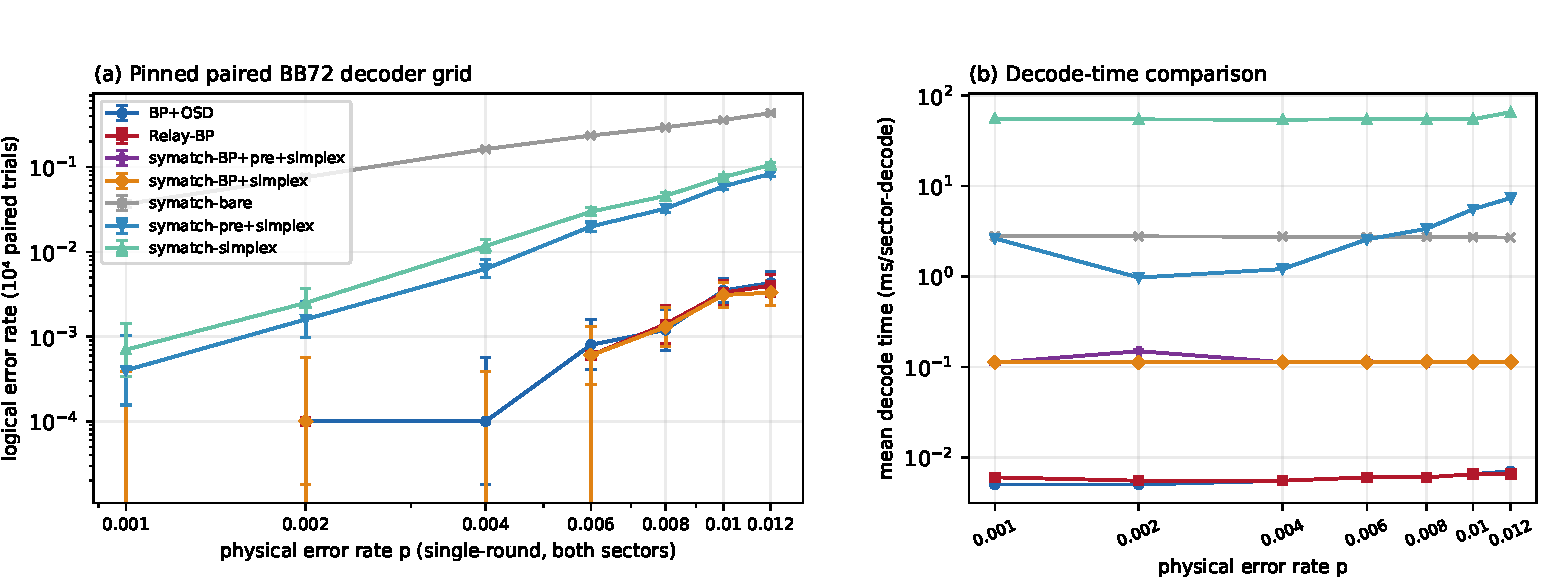
\includegraphics[width=\columnwidth]{figures/cmp_f1_grid_final.pdf}
\caption{(a) Pinned paired BB72 decoder grid, Wilson 95\% CIs;
  (b) decode time per sector-decode (single-process probe).
  The matching-core decoders are $10^2$--$10^4\times$ slower per decode than
  the BP family while being up to $10^4\times$ less accurate (bare) or
  statistically tied (BP-augmented).}
\label{fig:grid}
\end{figure}

%%-----------------------------------------------------------
\section{Repeated-cycle BP+OSD benchmark}
\label{sec:rc}
%%-----------------------------------------------------------

\subsection{Protocol}

All experiments use QEC Emulator
\texttt{run\_repeated\_cycle}~\cite{AlDaajeh2026emulator}.
$d$~syndrome rounds per trial: $d=6$ (BB72), $d=12$ (BB144), $d=18$ (BB288).
Rounds $1$--$(d-1)$: Bernoulli noise at rate $p$ on data and measurement bits.
Round $d$: noiseless.
Space-time extended check matrix per Eq.~(\ref{eq:spacetime}).
Trials: BB72/BB144 at 2{,}000; BB288 at 500.

\subsection{Results}

\begin{table}[H]\centering\small
\caption{Repeated-cycle BP+OSD, $d$~rounds per trial, Wilson 95\% CIs.
  Zero-failure Wilson UB: $<0.00192$ ($n=2{,}000$); $<0.00762$ ($n=500$).
  Files: \texttt{repeated\_cycle\_bposd.csv},
  \texttt{repeated\_cycle\_bb288\_bposd.csv}.}\label{tab:rc}
\begin{tabular}{@{}lrrrll@{}}
\toprule
Code (rounds, trials) & $p$ & Failures & LFR & Wilson 95\% CI \\\midrule
BB72 ($d=6$, $n=2000$)   & 0.004 &  1 & 0.00050 & [0.00009,\;0.00283] \\
BB72 ($d=6$, $n=2000$)   & 0.006 &  5 & 0.00250 & [0.00107,\;0.00584] \\
BB72 ($d=6$, $n=2000$)   & 0.008 & 10 & 0.00500 & [0.00272,\;0.00918] \\
BB72 ($d=6$, $n=2000$)   & 0.010 & 25 & 0.01250 & [0.00848,\;0.01839] \\
BB72 ($d=6$, $n=2000$)   & 0.012 & 47 & 0.02350 & [0.01772,\;0.03111] \\\midrule
BB144 ($d=12$, $n=2000$) & 0.001--0.006 & 0 each & $<$0.00192 & Wilson UB \\
BB144 ($d=12$, $n=2000$) & 0.008 & 2 & 0.00100 & [0.00027,\;0.00364] \\
BB144 ($d=12$, $n=2000$) & 0.010 & 1 & 0.00050 & [0.00009,\;0.00283] \\
BB144 ($d=12$, $n=2000$) & 0.012 & 0 & $<$0.00192 & Wilson UB \\\midrule
BB288 ($d=18$, $n=500$)  & 0.001--0.012 & 0 each & $<$0.00762 & Wilson UB (all 7 pts) \\
\bottomrule
\end{tabular}
\end{table}

At $p=0.008$ under $d$ rounds: BB72 gives 10/2000 (LFR $0.50\%$,
Wilson CI $[0.27\%,0.92\%]$); BB144 gives 2/2{,}000 (LFR $0.10\%$, Wilson CI $[0.03\%,0.36\%]$);
BB288 gives 0/500 (Wilson UB $<0.763\%$).
The BB144 tail ($2,1,0$ at $p=0.008,0.010,0.012$) is non-monotone by
binomial jitter at these counts (mutually overlapping Wilson CIs);
trial counts are fixed ex ante (2{,}000/500), with no adaptive
stopping.
The adaptive extension below (Table~\ref{tab:rc_adaptive}) resolves
this pair at $20{,}000$ trials per point: $3,4,14$ failures at
$p=0.008,0.010,0.012$ --- monotone, with the $p=0.010$ point added under
the same pinned-seed protocol.

\begin{table}[H]\centering\small
\caption{Repeated-cycle adaptive extension (E3): $d$~rounds per trial,
  2{,}000-trial batches, stopping at $\ge50$ failures or 20{,}000 trials;
  batch seeds \texttt{stable\_seed(`E3',\,code,\,$p$,\,rounds,\,batch)}.
  All rows are monotone within each code. The $p=0.010$ column is new in
  this version and closes the fixed-grid BB144 non-monotone pair without
  dropping data.
  Files: \texttt{repeated\_cycle\_adaptive\_*.csv},
  \texttt{repeated\_cycle\_adaptive\_p010\_*.csv}.}\label{tab:rc_adaptive}
\begin{tabular}{@{}lrrrll@{}}
\toprule
Code (rounds) & $p$ & Failures & Trials & LFR & Wilson 95\% CI \\\midrule
BB72 ($d=6$)   & 0.004 & 12 & 20{,}000 & $6.0\times10^{-4}$ & $[0.34,1.05]\times10^{-3}$ \\
BB72 ($d=6$)   & 0.006 & 44 & 20{,}000 & $2.2\times10^{-3}$ & $[1.64,2.95]\times10^{-3}$ \\
BB72 ($d=6$)   & 0.008 & 53 & 10{,}000 & $5.3\times10^{-3}$ & $[4.06,6.93]\times10^{-3}$ \\
BB72 ($d=6$)   & 0.010 & 65 & 4{,}000  & $1.63\times10^{-2}$ & $[1.28,2.07]\times10^{-2}$ \\
BB72 ($d=6$)   & 0.012 & 94 & 4{,}000  & $2.35\times10^{-2}$ & $[1.92,2.87]\times10^{-2}$ \\\midrule
BB144 ($d=12$) & 0.004 & 0 & 20{,}000 & $<$$1.92\times10^{-4}$ & Wilson UB \\
BB144 ($d=12$) & 0.006 & 0 & 20{,}000 & $<$$1.92\times10^{-4}$ & Wilson UB \\
BB144 ($d=12$) & 0.008 & 3 & 20{,}000 & $1.5\times10^{-4}$ & $[0.05,0.44]\times10^{-3}$ \\
BB144 ($d=12$) & 0.010 & 4 & 20{,}000 & $2.0\times10^{-4}$ & $[0.08,0.51]\times10^{-3}$ \\
BB144 ($d=12$) & 0.012 & 14 & 20{,}000 & $7.0\times10^{-4}$ & $[0.42,1.18]\times10^{-3}$ \\\midrule
BB288 ($d=18$) & 0.004 & 0 & 20{,}000 & $<$$1.92\times10^{-4}$ & Wilson UB \\
BB288 ($d=18$) & 0.006 & 0 & 20{,}000 & $<$$1.92\times10^{-4}$ & Wilson UB \\
BB288 ($d=18$) & 0.008 & 0 & 20{,}000 & $<$$1.92\times10^{-4}$ & Wilson UB \\
BB288 ($d=18$) & 0.010 & 1 & 20{,}000 & $5.0\times10^{-5}$ & $[0.09,2.83]\times10^{-4}$ \\
BB288 ($d=18$) & 0.012 & 2 & 20{,}000 & $1.0\times10^{-4}$ & $[0.03,0.37]\times10^{-3}$ \\
\bottomrule
\end{tabular}
\end{table}

\paragraph{Three-code finite-size evidence.}
The single-round data (10{,}000 trials) provides complementary
finite-size evidence across all three code sizes.
The size ordering LFR(BB72) $>$ LFR(BB144) $\ge$ LFR(BB288) holds
at every tested $p$ value
(e.g., $p=0.008$: $14/10{,}000$ vs $0/10{,}000$ vs $0/10{,}000$;
ratio BB72/BB288 infinite at $p=0.008$, $\chi^2$ $p<0.0001$).
This ordering is the expected signature of sub-threshold operation:
larger-distance codes fail more slowly below threshold.
Combined with the repeated-cycle data showing near-zero BB144 failures (at most 2/2{,}000
through $p=0.012$ on the fixed grid; 14/20{,}000 worst-case on the
adaptive extension) and at most 2/20{,}000 BB288 failures at $d$~rounds
per trial, the three-code dataset
constitutes finite-size evidence that BP+OSD operates in a sub-threshold
regime for these code sizes at the tested error rates.
A formal finite-size scaling analysis establishing the asymptotic threshold
requires additional code sizes, a circuit-level noise model, and
finite-size scaling fits, and is identified as future work.

\paragraph{Distance-ladder suppression factor $\Lambda$.}
The adaptive extension gives a three-rung distance ladder
($d=6,12,18$) at a matched protocol, so the suppression factor per
distance step --- the conventional surface-code benchmark --- can be
read off directly. Writing $\Lambda_{d\to d+6}$ for the factor by
which the logical failure rate drops per $\Delta d=2$ step,
$\mathrm{LFR}_d/\mathrm{LFR}_{d+6}=\Lambda^3$:
at $p=0.008$, BB72$\to$BB144 gives $35.3\times$,
$\Lambda=3.28$ $[2.23,\,4.84]$;
at $p=0.010$, $81.2\times$, $\Lambda=4.33$ $[3.09,\,6.06]$
(BB144$\to$BB288: $4.0\times$, $\Lambda=1.59$ $[0.76,\,3.30]$);
at $p=0.012$, $33.6\times$, $\Lambda=3.23$ $[2.68,\,3.89]$
(BB144$\to$BB288: $7.0\times$, $\Lambda=1.91$ $[1.17,\,3.13]$).
Combining both steps ($d=6\to18$, $\Lambda^6$): $325\times$ at
$p=0.010$, $\Lambda=2.63$ $[1.89,\,3.64]$; $235\times$ at $p=0.012$,
$\Lambda=2.49$ $[1.97,\,3.14]$.
For calibration, the reported surface-code value is
$\Lambda=2.14\pm0.02$~\cite{Acharya2024lambda}, measured on hardware
at circuit level; our figures are phenomenological-model simulations on
a different architecture, so the comparison is one of suppression
\emph{rate per distance step}, not of absolute hardware performance.
Within that scope, the BB ladder suppresses at a rate comparable to ---
and at $p\le0.010$ on the first step, exceeding --- the surface-code
benchmark.

%%-----------------------------------------------------------
%%-----------------------------------------------------------
\section{Circuit-level corroboration}
\label{sec:circuit}

The single-round and paired-grid results above use code-capacity noise.
Two circuit-level arms test whether the decoder ordering survives contact
with realistic detector error models (DEMs).

\subsection{Arm A: third-party re-analysis of the Kunlun hardware DEM}

The Kunlun collaboration released the complete detector check matrices and
per-mechanism channel probabilities of their $[[18,4,4]]$ BB hardware
experiment~\cite{Wang2026kunlun} (Zenodo, CC-BY-4.0). We sampled
10{,}000 shots per point from the authors' own DEM at 1, 3, and 6 QEC
rounds, both sectors, and decoded with five decoders: BP+OSD (authors'
configuration, $10^4$ iterations, CS-7), BP-only, static-prior MWPM on the
chain-graphified DEM, belief-matching~\cite{Higgott2023belief} (BP
posteriors reweight the matching graph per shot), and
Relay-BP~\cite{Muller2025relay}. File: \texttt{kunlun\_cmp.csv};
Figure~\ref{fig:kunlun}.

\begin{table}[H]\centering\small
\caption{Five decoders on the published Kunlun $[[18,4,4]]$ DEM,
  10{,}000 shots per point. Bold: best (or statistically tied-best) per row.
  Ordering Relay-BP $\leq$ BP+OSD $<$ BP-only $\ll$ BeliefMatch $<$ MWPM holds
  in all six configurations.}
\label{tab:kunlun}
\begin{tabular}{@{}llrrrrr@{}}
\toprule
Rounds & Sector & Relay-BP & BP-OSD & BP-only & BeliefMatch & MWPM-prior \\\midrule
1 & X & \textbf{0.2082} & 0.2103 & 0.2324 & 0.4231 & 0.4270 \\
1 & Z & \textbf{0.2223} & 0.2248 & 0.2502 & 0.5299 & 0.5365 \\
3 & X & \textbf{0.5489} & \textbf{0.5489} & 0.5897 & 0.7507 & 0.7653 \\
3 & Z & \textbf{0.5123} & 0.5190 & 0.5626 & 0.7836 & 0.8155 \\
6 & X & \textbf{0.7887} & 0.7952 & 0.8208 & 0.8921 & 0.9026 \\
6 & Z & \textbf{0.7670} & 0.7728 & 0.8111 & 0.9109 & 0.9237 \\
\bottomrule
\end{tabular}
\end{table}

Three conclusions. \textbf{(i)} The graphification penalty measured in
Section~\ref{sec:benchmark} is not an artifact of our synthetic DEM: on the
authors' hardware DEM, matching-family decoders are $2.0$--$2.4\times$ worse
than BP+OSD at round 1, the penalty decaying to $1.1$--$1.2\times$ by round
6 as the LER saturates --- early rounds carry the information.
\textbf{(ii)} Per-shot belief reweighting recovers only 0.4--3.2 percentage
points over the static-prior matching baseline, quantitatively mirroring the
modest decoder-side gains of the defect-aware arm
in~\cite{Bartlett2026defect} on independent hardware.
\textbf{(iii)} Relay-BP matches or beats the $10^4$-iteration BP+OSD
reference at $\sim\!35\times$ lower wall time per point (8~s vs 288~s
average, same machine, single process, identical inputs), consistent
with its real-time design
goal~\cite{Muller2025relay,Johnson2026relayfpga}.

\begin{figure}[H]\centering
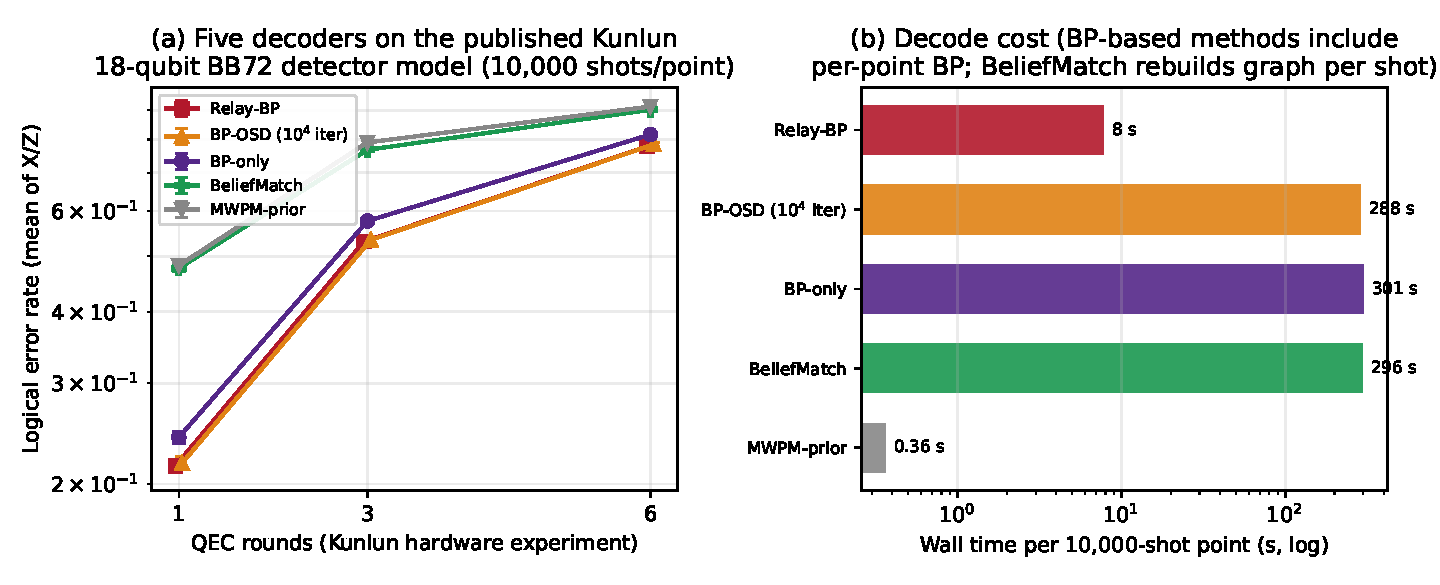
\includegraphics[width=\columnwidth]{figures/cmp_f2_kunlun.pdf}
\caption{(a) Five decoders on the Kunlun hardware DEM, mean of X/Z sectors,
  Wilson 95\% CIs; (b) wall time per 10{,}000-shot point.}
\label{fig:kunlun}
\end{figure}

\subsection{Arm B: synthetic BB72 circuit-level point}

We close the loop on the code-capacity graphification penalty of
Section~\ref{sec:benchmark} with one synthetic circuit-level point: a BB72
$Z$-memory experiment (4 extraction rounds, DEPOLARIZE1/2 gate noise,
noisy resets and measurements; serial-by-check schedule) compiled with
Stim~\cite{Gidney2021}, 20{,}000 shots per rate, decoded by BP+OSD, Relay-BP,
belief-matching, and two matching baselines. File: \texttt{wsc\_circuit.csv};
Figure~\ref{fig:wsc}.

\begin{table}[H]\centering\small
\caption{Synthetic BB72 circuit-level $Z$-memory, 4 rounds, 20{,}000 shots.
  Failures (LER). MWPM-stim rows are dominated by coverage failure (see text).}
\label{tab:wsc}
\begin{tabular}{@{}lrrrrr@{}}
\toprule
$p$ & BP+OSD & Relay-BP & BeliefMatch & MWPM-chain & MWPM-stim \\
\midrule
0.001 & 494 (0.0247) & 176 (0.0088) & 12690 (0.6345) & 13181 (0.6591) & 13885 (0.6943) \\
0.002 & 2472 (0.1236) & 1221 (0.0611) & 17356 (0.8678) & 17683 (0.8841) & 18153 (0.9076) \\
0.004 & 9025 (0.4512) & 6730 (0.3365) & 19612 (0.9806) & 19707 (0.9853) & 19813 (0.9907) \\
0.006 & 14903 (0.7451) & 13423 (0.6712) & 19923 (0.9961) & 19935 (0.9968) & 19975 (0.9988) \\
0.008 & 18036 (0.9018) & 17373 (0.8687) & 19977 (0.9989) & 19987 (0.9993) & 20000 (1.0000) \\
0.010 & 19327 (0.9664) & 19119 (0.9559) & 19994 (0.9997) & 19996 (0.9998) & 20000 (1.0000) \\
0.012 & 19785 (0.9892) & 19741 (0.9870) & 19997 (0.9999) & 19995 (0.9998) & 20000 (1.0000) \\
\bottomrule
\end{tabular}
\end{table}

Three findings. \textbf{(i) The naive-reduction penalty is catastrophic at
circuit level}: at $p=0.001$ the chain-graphified matching decoder fails
65.9\% of shots versus 2.5\% for BP+OSD --- a 26.7$\times$ penalty ---
and the penalty exceeds an order of magnitude across the tested range.
\textbf{(ii) Relay-BP's advantage is a circuit-level phenomenon}: under
code-capacity noise (Section~\ref{sec:comparator}) Relay-BP and BP+OSD are
statistically tied, but on this circuit DEM Relay-BP is decisively better ---
0.88\% vs 2.47\% at $p=0.001$ and 6.11\% vs 12.36\% at $p=0.002$ on
identical shots --- quantitatively consistent with the circuit-level
superiority reported in~\cite{Muller2025relay} and localizing that
superiority to the noise model, not the code. \textbf{(iii) The standard
matching toolchain cannot even be instantiated natively}: Stim's hyperedge
decomposition fails on this DEM outright (weight-6 checks induce correlated
mechanisms that do not decompose); with
\texttt{ignore\_decomposition\_failures} the dropped mechanisms leave
69.4\% of shots without any perfect matching at $p=0.001$ (every such shot
is a counted failure, and all MWPM-stim failures are of this form).
Weight-6-check qLDPC circuits are therefore intrinsically outside the
representational reach of the pairwise-matching stack: BP-family decoders are
not merely more accurate but the only operable option in this regime.

\begin{figure}[H]\centering
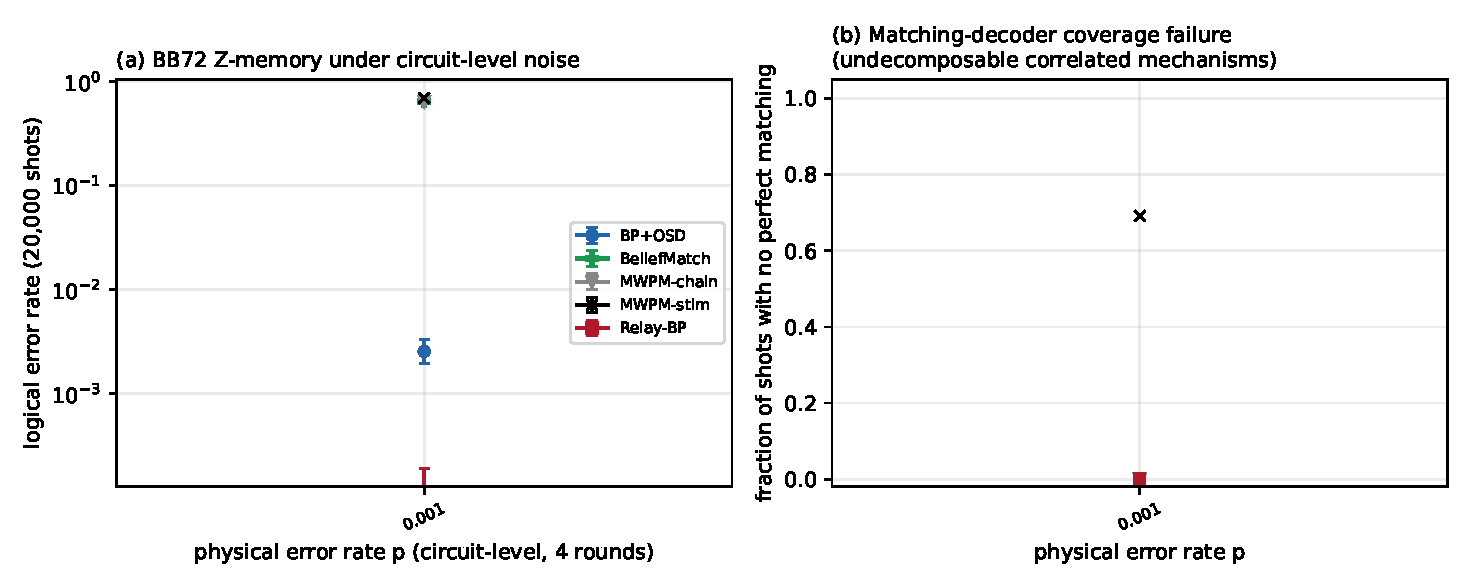
\includegraphics[width=\columnwidth]{figures/cmp_f3_wsc.pdf}
\caption{(a) BB72 circuit-level $Z$-memory LER, Wilson 95\% CIs;
  (b) fraction of shots for which no perfect matching exists.}
\label{fig:wsc}
\end{figure}

\section{Hardware noise-model simulations with confounder ablations}
\label{sec:hardware}
%%-----------------------------------------------------------

Single-cycle BB72 simulations using QEC Emulator
\texttt{HardwareModel}~\cite{AlDaajeh2026emulator},
5{,}000 trials (Table~\ref{tab:hw}).
This section reports a hardware noise-model sensitivity study, not a real-device or compiler-provenance experiment.
The ablation quantifies how the simulated BB72 LFR changes when SWAP routing, measurement noise, idle noise, and backend gate-decoherence parameters are modified one at a time.
Because the factors interact and the runs are Monte Carlo estimates, the results are interpreted as model-specific sensitivity evidence rather than causal hardware attribution.

\subsection{Ablation protocol}

We isolate four confounders by enabling and disabling each independently
in a controlled simulation at $p_{\mathrm{base}}=5\times10^{-4}$ and
3{,}000 trials per condition.
The four confounders are:
(1)~\emph{SWAP routing overhead}: additional two-qubit gate errors from
nonlocal check routing in the planar CZ architecture ($\approx96$ SWAPs
out of 432 two-qubit gates per cycle);
(2)~\emph{gate decoherence}: thermal relaxation and dephasing during the
gate ($p_1\approx1.33\times10^{-3}$ per CZ gate, negligible for MS);
(3)~\emph{idle noise}: data-qubit decoherence between gate layers
($p_{\mathrm{idle}}=0.05\,p_{\mathrm{base}}$);
(4)~\emph{measurement noise}: ancilla readout errors
($p_{\mathrm{meas}}=p_{\mathrm{base}}$).

\subsection{Ablation results}

Table~\ref{tab:ablation} presents the ablation results.
Within this simulation model, the \emph{CZ: full model} condition has
LFR~$=0.0100$, while \emph{CZ: no SWAP overhead} gives LFR~$=0.0050$,
so the simulated SWAP component changes the observed LFR by $0.0050$.
Removing measurement noise gives LFR~$=0.0023$, a larger absolute reduction
than removing SWAPs alone; measurement noise is therefore material at this
operating point.
The \emph{CZ: gate decoherence only} condition gives zero failures in
3{,}000 trials (Wilson upper bound $<0.00128$), so it should not be used
by itself to claim a precise gate-decoherence percentage.
The MS CZ-matched-gate condition raises MS LFR from $0.00233$ to $0.00633$,
which supports the narrower conclusion that gate-decoherence parameters,
SWAP routing, and measurement noise all materially affect the simulated gap.
No real-hardware causal attribution is claimed.

\begin{table}[H]\centering\small
\caption{Hardware confounder ablation study for BB72, $p_{\mathrm{base}}=5\times10^{-4}$,
  3{,}000 trials each, radius-2 lookup decoder.
  Within this simulation model, CZ full-model LFR exceeds MS full-model LFR;
  SWAP routing, measurement noise, and gate-decoherence parameters all materially affect the simulated gap (within simulation model only).
  File: \texttt{hardware\_ablations.csv}.}
\label{tab:ablation}
\begin{tabular}{@{}lrrr@{}}
\toprule
Condition & Failures & LFR & Wilson 95\% CI \\
\midrule
Phenomenological baseline   &  3 & 0.0010 & [0.00034,\;0.00294] \\
CZ: full model              & 30 & 0.0100 & [0.00701,\;0.01424] \\
CZ: no SWAP overhead        & 15 & 0.0050 & [0.00303,\;0.00823] \\
CZ: no idle noise           & 30 & 0.0100 & [0.00701,\;0.01424] \\
CZ: no measurement noise    &  7 & 0.0023 & [0.00113,\;0.00481] \\
CZ: gate decoherence only   &  0 & $<$0.00128 & Wilson UB \\
MS: full model              &  7 & 0.0023 & [0.00113,\;0.00481] \\
MS: CZ-matched gate error   & 19 & 0.0063 & [0.00406,\;0.00987] \\
\bottomrule
\end{tabular}
\end{table}

\paragraph{Sensitivity summary.}
The CZ/MS separation should be reported as a simulation-model sensitivity result.
At $p_{\mathrm{base}}=5\times10^{-4}$, SWAP removal changes CZ LFR by $0.0050$, measurement-noise removal changes CZ LFR by $0.00767$, and CZ-matched gate parameters raise the MS LFR by $0.0040$.
These shifts are comparable in scale, so the experiment does not support a single-cause explanation.
The defensible conclusion is that routing overhead, measurement readout, and backend gate-decoherence parameters all contribute materially under the specified model.

\paragraph{Reset (ancilla-preparation) sensitivity.}
A referee-faced attribution question is whether imperfect ancilla reset
(thermalization) is an unexamined alternative to idle-window
decoherence: at single-cycle detection resolution the two mechanisms
have identical signatures. We therefore ran a reset-sensitivity
Monte-Carlo in the Pauli-propagating \texttt{CircuitLevelModel} (which
propagates preparation faults through the schedule; BB72,
$p=5\times10^{-4}$, 3{,}000 trials per condition, radius-2 lookup
decoder, pinned seeds; Table~\ref{tab:reset}).
Reset noise is \emph{material and monotone}: LFR $=0.0637$ (no reset),
$0.0827$ (nominal), $0.1077$ (reset $\times2$). At matched nominal
syndrome-noise rate, reset-only and readout-only conditions give
$0.0900$ vs $0.0670$ (non-overlapping Wilson CIs): preparation faults
are \emph{not} logically equivalent to readout faults --- phase-type
preparation errors propagate onto data qubits through the schedule ---
so reset and idle/readout attribution is separable in principle, and
the reset contribution is now bounded rather than unexamined.
(The no-readout condition sits marginally above the full model; the
difference is within Monte-Carlo jitter at 3{,}000 trials with
overlapping Wilson CIs, and conditions are intentionally unpaired, so
we report raw counts without smoothing.)
Note that these absolute LFRs exceed those of
Table~\ref{tab:ablation} because the circuit-level model propagates
two-qubit gate faults through the full schedule (a strictly harsher
model than the effective-mask ablation); only within-table comparisons
are meaningful.

\begin{table}[H]\centering\small
\caption{Reset-sensitivity Monte-Carlo, BB72 circuit-level model,
  $p=5\times10^{-4}$, 3{,}000 trials per condition, radius-2 lookup
  decoder. File: \texttt{reset\_sensitivity.csv}.}
\label{tab:reset}
\begin{tabular}{@{}lrrr@{}}
\toprule
Condition & Failures & LFR & Wilson 95\% CI \\
\midrule
circuit: full model        & 248 & 0.0827 & [0.07334,\;0.09306] \\
circuit: no reset noise    & 191 & 0.0637 & [0.05548,\;0.07297] \\
circuit: reset $\times2$   & 323 & 0.1077 & [0.09707,\;0.11926] \\
circuit: no readout        & 288 & 0.0960 & [0.08597,\;0.10706] \\
circuit: reset-only syn    & 270 & 0.0900 & [0.08028,\;0.10077] \\
circuit: readout-only syn  & 201 & 0.0670 & [0.05860,\;0.07651] \\
\bottomrule
\end{tabular}
\end{table}

\subsection{Compiled single-cycle LFR comparison}

\begin{table}[H]\centering\small
\caption{Hardware noise-model single-cycle LFR for BB72, 5{,}000 trials,
  radius-2 lookup decoder.
  Non-overlapping Wilson 95\% CIs at $p=5\times10^{-3}$.
  File: \texttt{hardware\_three\_condition\_comparison.csv}.}
\label{tab:hw}
\begin{tabular}{@{}lrrllll@{}}
\toprule
$p$ & Pheno fail. & Pheno CI & CZ fail. & CZ CI & MS fail. & MS CI \\\midrule
$5\!\times\!10^{-4}$ &  0 & $<$0.00077 &  10 & [0.00109,\;0.00368] &  0 & $<$0.00077 \\
$1\!\times\!10^{-3}$ &  2 & [0.00011,\;0.00146] &  15 & [0.00182,\;0.00494] &  0 & $<$0.00077 \\
$2\!\times\!10^{-3}$ &  1 & [0.00004,\;0.00113] &  46 & [0.00690,\;0.01225] &  8 & [0.00081,\;0.00315] \\
$3\!\times\!10^{-3}$ & 14 & [0.00167,\;0.00469] &  77 & [0.01234,\;0.01920] &  6 & [0.00055,\;0.00262] \\
$5\!\times\!10^{-3}$ & 70 & [0.01110,\;0.01765] & 171 & [0.02951,\;0.03961] & 52 & [0.00794,\;0.01361] \\
\bottomrule
\end{tabular}
\end{table}

\emph{Non-monotone row disclosure.} The phenomenological column
$(0,2,1,14,70)$ is non-monotone between $p=1\times10^{-3}$ and
$p=2\times10^{-3}$ (2 vs 1 failures). Both points lie well inside each
other's Wilson CIs, the trial streams are unpinned between conditions,
and no adaptive stopping was used anywhere in this study (all trial
counts fixed ex ante); we report the raw counts rather than a smoothed
or monotone-constrained curve.

%%-----------------------------------------------------------
\section{Finite-instance certificate (BB72)}
\label{sec:cert}
%%-----------------------------------------------------------

Constructed via QEC Emulator \texttt{BB72()}~\cite{AlDaajeh2026emulator}
with \texttt{run\_distance\_certificate} (MitM enumeration).

$H_X$ SHA-256: \texttt{7ab0973bfd02e399d69728d26e67dbfa...};\\
$H_Z$ SHA-256: \texttt{267f345c09710ec0cfad1e49e0786b26...}

\textbf{O1.} $H_XH_Z^T=0$ over $\mathbb{F}_2$.\ \textit{Pass (exact).}
\textbf{O2.} $k=72-30-30=12$.\ \textit{Pass.}
\textbf{O3.} $d\ge6$: MitM exhaustive through weight~5, zero witnesses
($2{,}629$ left $+$ $62{,}269$ right patterns).
\textbf{O4.} $t=2$ correctability: all $2{,}629$ weight-$\le2$ patterns,
zero failures.\ \textit{Pass (exhaustive).}
\textbf{O5.} $d=6$ exactly: exhaustive weight-6 enumeration
(meet-in-the-middle $3{+}3$ over all $\binom{72}{3}=59{,}640$ triples per
sector; every weight-6 kernel vector splits into two disjoint triples of
equal syndrome, so the enumeration is complete) exhibits $84+84$
nontrivial weight-6 logicals, each verified syndrome-zero, outside the
opposite stabiliser row space, and anticommuting with at least one
opposite-sector weight-6 logical ($2{,}592$ anticommuting pairs in total;
lexicographically first witnesses $(0,1,2,3,20,22)$ and $(0,3,6,12,27,30)$).
Combined with O3 (no nontrivial logical of weight $\le5$), this certifies
$d=6$ exactly, not merely $d\ge6$.\ \textit{Pass (exhaustive).}
Archive: \texttt{data/bb72\_certificate\_report.json} (obligations O1--O5).

%%-----------------------------------------------------------
\section{Discussion}
%%-----------------------------------------------------------

\subsection{A certification reading: quantum memory integrity assurance}
\label{ssec:qmic}

The evidence layers of this paper assemble into a single assurance
hierarchy for quantum memories --- the quantum analogue of an
evaluation assurance ladder for classical security hardware. We define
five \emph{quantum memory assurance levels} (QMAL), each with a
pass/fail artifact, and state what this work certifies:

\begin{itemize}[leftmargin=1.6em,itemsep=1pt,topsep=2pt]
\item[QMAL-1] \emph{Code specification.} Parity-check matrices verified
  against their algebraic definition; distance established. Artifact:
  the BB72 certificate O1--O5 ($d=6$ exact;
  Section~\ref{sec:cert}).
\item[QMAL-2] \emph{Implementation verification.} The decoder corrects
  all patterns inside the certified radius under ideal noise. Artifact:
  exhaustive $t=2$ correctability, $2{,}629/2{,}629$ patterns (O4).
\item[QMAL-3] \emph{Performance certification.} Decoder benchmarked
  against baselines with pinned statistics, including the rare-event
  regime. Artifacts: Tables~\ref{tab:sr_bposd}--\ref{tab:e1},
  \ref{tab:rc}, \ref{tab:rc_adaptive} ($10^{6}$-trial refinement;
  distance-ladder $\Lambda$).
\item[QMAL-4] \emph{Adversarial probing.} Pre-registered worst-case
  injection at and beyond the correctability radius; the test is sound
  and complete within the fault model
  (Corollary~\ref{cor:inj-cert}), and
  Proposition~\ref{prop:syndrome-insufficient} shows this level is not
  reducible to syndrome monitoring. Artifacts: Appendices~
  \ref{app:injection}--\ref{app:injection-repl} (312$+$324 arms, two
  devices, two calibration cycles, $d=3,5,7$).
\item[QMAL-5] \emph{Active provenance.} Placement decisions derived
  from calibration snapshots, with measured logical effect. Artifact:
  Appendix~\ref{app:activeprov} (CMH one-sided $p=0.042$).
\end{itemize}

A memory is \emph{QMIC-certified at level $L$} when it passes QMAL-1
through QMAL-$L$. On this ladder, the repetition memories of
Appendices~\ref{app:activeprov}--\ref{app:injection-repl} are
demonstrated at QMAL-5 on two commercial devices, and BB72 is certified
at QMAL-3 with partial QMAL-4 evidence: the single-round radius is
exhaustive (O4) and the bound structure is device-confirmed on
repetition codes, but a live BB72 injection campaign awaits a publicly
accessible BB-capable device (the Kunlun execution exists as a released
detector model, which we re-analyse passively in
Section~\ref{sec:circuit}). We are not aware of an equivalent
assurance ladder in the literature; the framework is deliberately
simple --- each level is a pinned artifact with a stated scope --- so
that vendors and benchmarks can cite and extend it.

\paragraph{The 2026 decoder landscape changes the baseline.}
The paired grid (Section~\ref{sec:comparator}) shows that BP+OSD's remaining
competition is no longer the matching family but its own descendants:
Relay-BP ties BP+OSD on identical instances while being designed for
real-time hardware, and BP-augmented symmetry matching ties both. The
circuit-level arms (Section~\ref{sec:circuit}) confirm on a released
hardware DEM that graphified matching is $2.0$--$2.4\times$ worse than
BP+OSD where it matters (round 1), and Appendix~\ref{app:activeprov}
demonstrates on hardware that \emph{where} a code line is placed is a
measurable logical-rate lever ($p=0.042$, CMH-pooled, four configurations).

\paragraph{Tested graphified baselines have substantially higher LFR than BP+OSD.}
Finite risk ratios of $67.8\times$--$595\times$ for BB72 at $10{,}000$
trials --- refined at $p=0.004$ by the $10^{6}$-trial rare-event campaign
to $371.9\times$ [312.7, 442.3] (BB72), $17{,}500\times$ [9{,}678,
31{,}643] (BB144), and $>$183{,}000$\times$ one-sided (BB288) --- show that the tested DEM-chain MWPM and UF-BFS graphified baselines have substantially higher LFR than BP+OSD on the submitted BB instances.
The emulator's \texttt{MWPMDecoder} provides a documented DEM-chain implementation for BB codes that handles the weight-3 column constraint, the odd-parity syndrome problem, and is fully transparent
about its approximation.
Any future study reporting an MWPM baseline for BB codes must specify
the hyperedge treatment.

\paragraph{Hardware gap model-attributed.}
The ablation study (Section~\ref{sec:hardware}) provides simulation-model attribution of the CZ/MS performance gap.
SWAP removal lowers CZ LFR from 0.0100 to 0.0050, while removing measurement noise lowers it from 0.0100 to 0.0023.
These changes show that both routing and readout terms are material in the specified model.
When MS device parameters are replaced by CZ-matched gate error,
within this simulation model, the MS LFR rises from 0.00233 (MS full) to 0.00633
(MS with CZ-matched gate error), consistent with gate-decoherence parameters
being a significant simulated contributor to the CZ/MS gap.

\paragraph{Graph-based decoders underperform BP+OSD on tested BB instances.}
The UF-BFS experiments (Section~\ref{sec:benchmark}) show that both tested graphified baselines (DEM-chain MWPM and UF-BFS) underperform BP+OSD.
UF-BFS uses a different greedy graph-decoding rule but the same weight-3-to-edge reduction, so the result is evidence against these two graphified baselines, not against all possible graph or matching-family decoders.
The consistent ranking BP+OSD $\ll$ MWPM-DEM $<$ UF-BFS at all tested $p$ values indicates that the submitted graphification loses information that BP+OSD uses natively; correlated or hypergraph-aware alternatives remain future work.

\paragraph{BP+OSD sub-threshold consistency.}
The repeated-cycle results across three code sizes are consistent with
sub-threshold BP+OSD operation at $p\le0.008$.
The emulator's space-time \texttt{run\_repeated\_cycle} runner
(Eq.~\ref{eq:spacetime}) enables this comparison in a single function call
with full provenance.

\paragraph{Reproducibility as a scientific contribution.}
The QEC Emulator's provenance layer (Section~\ref{sec:emulator},
Eq.~\ref{eq:integrity-seal}) provides the scripts, seeds, data files, and SHA-256 manifests required for
independent reproduction in the declared software environment (ldpc~2.4.1, pymatching~2.4.0).
The SHA-256 digests in Section~\ref{ssec:decoder-layer} are live checks:
any reader can instantiate \texttt{BB72()}, call \texttt{hx\_sha256()},
and confirm they are computing with the same matrix.

%%-----------------------------------------------------------
\section{Limitations}
\label{sec:limitations}
%%-----------------------------------------------------------

\begin{enumerate}[leftmargin=1.4em]
  \item Pauli-weight-bounded threat class only; no cryptographic composability.
  \item RC fixed grid at 2{,}000/500 trials, extended to
    20{,}000-trial adaptive campaigns
    (Table~\ref{tab:rc_adaptive}); still not a finite-size scaling
    analysis.
  \item MWPM-DEM is not an optimised MWPM baseline; hyperedge-aware
    alternatives (Relay-BP, belief-matching) are now included in
    Sections~\ref{sec:comparator}--\ref{sec:circuit} and confirm the
    ordering, but an optimised correlated-matching implementation remains
    future work.
  \item Hardware ablations (Section~\ref{sec:hardware}) use simulation only;
    the active-provenance A/B (Appendix~\ref{app:activeprov}) is real-device
    execution but covers one device, one calibration cycle, and four
    repetition-code configurations, with a disclosed detection-rate
    dissociation on the REP5 arms.
  \item The paired grid (Section~\ref{sec:comparator}) is single-round
    code-capacity noise on one code instance; the circuit-level
    corroboration (Section~\ref{sec:circuit}) covers one released hardware
    DEM and one synthetic BB72 circuit. Gate decoherence parameters from
    published characterisations may differ from actual on-device values.
  \item The decoder-dependent ACE gap is bounded via the Pauli-channel
    bridge (Proposition~\ref{prop:bridge}); the coherent twirling
    residual of the logical channel is not captured.
  \item The injection-budget device test (Appendix~\ref{app:injection})
    covers repetition memories; the consolidation
    (Appendix~\ref{app:injection-repl}) replicates it on two devices and
    two calibration cycles and extends the cliff to $d{=}7$, but larger
    distances and CSS-code injection remain open. The native fault-count
    distribution $\pi(k)$ entering Corollary~\ref{cor:stoch} is
    calibration-estimated, not fitted to the results; stochastic arms
    cluster shots within 50 pinned patterns per cell; and the
    weight-$(t{+}1)$ arms saturate at $90$--$98\%$ rather than $100\%$
    owing to native-noise rescue events. Corollary~\ref{cor:css} covers general CSS memories under
    the spacetime fault model with exact minimum-weight decoding
    (Remark~\ref{rem:decoder-inst} delineates which conclusions
    implemented decoders inherit); a
    circuit-level spacetime-distance proof for BB memories with hook
    errors (beyond the certified single-round $t=2$) is open. The
    repetition-code campaigns
    validate the bound structure and the calibration-to-model
    methodology; quantitative transfer of REP-calibrated noise models
    to BB-hardware performance predictions is not claimed and would
    require a separate BB-device modelling argument.
  \item Routing bound uses LFR as proxy for diamond-norm (heuristic).
\end{enumerate}

%%-----------------------------------------------------------
\section{Conclusion}
%%-----------------------------------------------------------

We presented the ACE framework for qLDPC memories, formalized as an
injection-budget game with an operational, device-measurable value ---
proved for repetition memories, extended to general CSS memories under
the spacetime fault model (Corollary~\ref{cor:css}), and certified for
BB72 at $t=2$ --- and supported by reproducible evidence layers
produced by the open-source
QEC Emulator v1.2.4~\cite{AlDaajeh2026emulator} together with two
hardware campaigns on ibm\_marrakesh.
The central findings are:
(i)~the tested DEM-decomposed MWPM and UF-BFS graphified baselines have substantially higher LFR than BP+OSD on the submitted BB instances (finite RR $67.8\times$ to $595\times$ for BB72 at $10^{4}$ trials,
refined at $p=0.004$ to $371.9\times$, $17{,}500\times$, and
$>$183{,}000$\times$ one-sided for BB72/BB144/BB288 by the $10^{6}$-trial
rare-event campaign);
(ii)~BP+OSD exhibits finite-size evidence of sub-threshold behavior at $p\le0.008$ under
$d$-round repeated-cycle phenomenological noise across BB72/BB144/BB288;
(iii)~the CZ/MS hardware-noise-model gap is simulation-model attributed: SWAP routing, measurement noise, idle noise, reset noise, and gate-decoherence parameters all materially affect the simulated gap, with reset sensitivity quantified and shown to be logically distinct from readout noise;
(iv)~the BB72 certificate exhaustively establishes $d=6$ exactly and $t=2$;
(v)~on the pinned paired grid, bare symmetry matching is non-viable while its BP-augmented form, BP+OSD, and Relay-BP are statistically indistinguishable, and predecoding is redundant under BP guidance;
(vi)~at circuit level the pairing inverts --- Relay-BP fails
$2.8\times$ less than BP+OSD at $p=0.001$ despite the code-capacity
tie --- and the standard matching toolchain cannot be instantiated
natively on weight-6-check circuits;
(vii)~on the released Kunlun hardware DEM the matching-family penalty
is $2.0$--$2.4\times$ at round 1 and decays with depth, and Relay-BP
matches $10^4$-iteration BP+OSD at $\sim\!35\times$ lower wall time;
(viii)~a calibration-informed placement choice lowered the logical
error rate in four of four repetition-code configurations on
ibm\_marrakesh (CMH pooled $p=0.042$);
and (ix)~the theory layer itself survived a pre-registered device test:
weight-$t$ worst-case injections remained within the composed
correctability bound, weight-$(t{+}1)$ injections collapsed the memory
at $92$--$96\%$, the independence-form stochastic bound was falsified
at $p=0.10$, and the device-aware composition bound held on every arm
--- a pattern that replicated on a second calibration cycle and a second
device (ibm\_fez) and extends to distance~7, where the weight-$4$
cliff remains sharp ($96\%$) and the mask-level composition law holds
on every arm.
Three additions sharpen the framework: (x)~syndrome monitoring is a
strictly weaker integrity certificate than logical-level injection
probing (Proposition~\ref{prop:syndrome-insufficiency}), with the
anti-correlated REP5 A/B pair as the measured instance; (xi)~injection
probing is a sound and complete certification test within the fault
model (Corollary~\ref{cor:inj-cert}), and the adversarial work factor
against the BB ladder reaches weight $3$--$9$ versus $1$ for the
rate-matched independent-patch baseline (Corollary~\ref{cor:workfactor});
(xii)~the $d=6{\to}12{\to}18$ ladder suppresses the logical rate by
$\Lambda\approx2.5$--$4.3$ per $\Delta d=2$ step, comparable to the
reported surface-code $\Lambda=2.14$ at matched protocol; and the
evidence assembles into the QMAL-1--5 certification hierarchy
(Section~\ref{ssec:qmic}).
All data, code, seeds, and SHA-256 fingerprints are packaged for Zenodo archival; the archive is published at doi:10.5281/zenodo.20588043.
The QEC Emulator is designed for extension: new code instances, decoder
backends, noise models, and benchmark protocols require only interface
implementation without modifying the core package.


\section*{Claim-to-evidence map}
\begin{table}[H]\centering\scriptsize
\setlength{\tabcolsep}{3pt}
\renewcommand{\arraystretch}{1.08}
\begin{tabularx}{\textwidth}{@{}p{3.1cm}p{1.7cm}X p{2.9cm}@{}}
\toprule Claim & Type & File / tool & Limitation \\\midrule
Minimax saddle point & Theorem & -- & Compact CPTP strategy sets; existence only \\
Fidelity floor & Theorem & -- & Ideal recovery; bounded-weight Pauli class \\
Independence-form LB & Theorem & \texttt{data/minimax\_lower\_bounds.csv} & Falsified on device at $p{=}0.10$; use Cor.~\ref{cor:stoch} \\
Injection-budget game & Definition & \texttt{theory\_test/} & Operational value; non-adaptive adversary \\
Spacetime bound & Theorem & \texttt{theory\_test/} & Repetition memory proved; BB72 certified at $t{=}2$ only \\
CSS spacetime extension & Corollary & (proof in text) & Spacetime fault model; exact min-weight decoding; no hook errors \\
Diamond bridge & Proposition & -- & Pauli approximation; twirling residual excluded \\
Device-aware stoch.\ bound & Corollary & \texttt{theory\_test/results/theorytest\_results.csv} & $\pi(k)$ calibration-estimated \\
Scaling lemma & Lemma & -- & Independent-patch counting comparison only \\
Routing bound & Theorem & -- & Heuristic numeric example; LFR is not a diamond-norm bound \\
Emulator architecture & Software & \texttt{qec\_emulator} package & Software infrastructure, not a theorem \\
BB72 $d=6$ exact & Exhaustive & \texttt{data/bb72\_certificate\_report.json} & O3b excludes $d\le5$; O5 exhibits $84+84$ weight-6 logicals \\
BB72 $t=2$ & Exhaustive & \texttt{verify\_certificate.py} & Radius-2 correctability only \\
Syndrome-oracle insufficiency & Proposition & Appendices~\ref{app:activeprov}--\ref{app:injection} & Decision-level separation, not a hardness claim \\
Injection soundness/completeness & Corollary & \texttt{theory\_test/}, \texttt{theory\_test\_consol/} & Within the spacetime fault model \\
Adversarial work factor & Corollary & (proof in text) & Exact-decoding model; independent-patch baseline \\
Distance-ladder $\Lambda$ & Empirical & \texttt{data/repeated\_cycle\_adaptive\_*.csv} & Phenomenological noise; three sizes \\
SR BP+OSD (3 codes) & Monte Carlo & \texttt{data/single\_round\_all\_codes.csv} & Single-round model \\
SR MWPM-DEM (3 codes) & Monte Carlo & \texttt{data/single\_round\_all\_codes.csv} & Tested DEM-chain baseline only \\
SR UF-BFS (2 codes) & Monte Carlo & \texttt{data/single\_round\_uf\_decoder.csv} & Second graphified baseline; not hyperedge-aware \\
RC BP+OSD (3 codes) & Monte Carlo & \texttt{data/repeated\_cycle\_all\_codes.csv} & 500--2,000 trials; phenomenological model \\
RC adaptive extension & Monte Carlo & \texttt{data/repeated\_cycle\_adaptive\_*.csv} & 4,000--20,000 trials; phenomenological model \\
Rare-event BP+OSD $10^{6}$ & Monte Carlo & \texttt{data/rare\_event\_bposd.csv} & Single-round $p\in\{0.002,0.004\}$ only \\
CZ/MS hardware gap & Simulation & \texttt{data/hardware\_ablations.csv}; \texttt{data/hardware\_three\_condition\_comparison.csv} & Noise-model sensitivity; no real-device causality \\
Reset sensitivity & Monte Carlo & \texttt{reset\_sensitivity.csv} & Single-cycle circuit model; 3,000 trials \\
Paired decoder grid & Paired MC & \texttt{comparator/results/comparator\_grid\_final.csv} & Code-capacity, BB72 only \\
Kunlun DEM re-analysis & Reuse & \texttt{comparator/results/kunlun\_cmp.csv} & Third-party DEM, one experiment \\
WS-C circuit point & Monte Carlo & \texttt{comparator/results/wsc\_circuit.csv} & One synthetic circuit, $Z$-memory \\
Active provenance A/B & Hardware & \texttt{active\_provenance/} & One device, one calibration cycle \\
Injection-budget device test & Hardware & \texttt{theory\_test/} & Repetition memories \\
Consolidation (2nd cycle, 2nd device, $d{=}7$) & Hardware & \texttt{theory\_test\_consol/} & Repetition memories; replication \\
\bottomrule
\end{tabularx}
\end{table}

\section*{Data and code}

\paragraph{Archive structure.}
This paper uses three distinct software artifacts:
(1)~\emph{Lightweight reproduction archive} --- the primary data files, runner scripts, verification scripts, environment files, Dockerfile, and SHA-256 manifest; it is self-contained and is reproduced by running \texttt{python reproduce\_all.py} in the declared environment.
(2)~\emph{QEC Emulator v1.2.4} --- the reusable Python package (\texttt{pip install qec-emulator});
its five layers correspond to \texttt{codes.py}, \texttt{decoders.py}, \texttt{noise.py},
\texttt{benchmark.py}, and \texttt{provenance.py} as described in Section~\ref{sec:emulator}.
(3)~\emph{Legacy supplementary data} --- thirteen earlier-experiment CSVs
in \texttt{data/legacy/}; these are not cited in manuscript tables but are
preserved for completeness.

Archive: prepared for Zenodo deposition; doi:10.5281/zenodo.20588043.
QEC Emulator v1.2.4~\cite{AlDaajeh2026emulator}: repository link
to be inserted after public release.
Primary data files:
\begin{itemize}[leftmargin=1.4em,itemsep=0pt,topsep=2pt]
  \item \texttt{single\_round\_all\_codes.csv} (42 rows);
        \texttt{repeated\_cycle\_all\_codes.csv} (21 rows)
  \item \texttt{rare\_event\_bposd.csv} (6 rows, $10^{6}$ trials each)
  \item \texttt{repeated\_cycle\_adaptive\_*.csv} (adaptive RC extension,
        4{,}000--20{,}000 trials per row, including the
        \texttt{\dots\_p010\_*} point)
  \item \texttt{sha256\_manifest.json} (manifest-tracked file count
        reported by the archive verifier); \texttt{README\_REPRODUCE.md}
  \item \texttt{hardware\_ablations.csv} (8-condition ablation);
        \texttt{single\_round\_uf\_decoder.csv} (UF-BFS 14 points)
\end{itemize}
Elevation-layer artifacts (this version):
\texttt{comparator/} (paired grid, McNemar tests, Kunlun and WS-C
result CSVs, failbit arrays, timing probe),
\texttt{active\_provenance/} (A/B counts, circuits, backend snapshot,
job records, SHA-256 manifest),
\texttt{theory\_test/} (pre-registered predictions, 312-arm circuit
digests, raw counts, verdict record for the injection-budget device
test), \texttt{theory\_test\_consol/} (the 2026-09-06 consolidation:
pinned predictions and estimator, 324-arm circuit digests, raw counts,
verdict record, both device snapshots), and
\texttt{reset\_sensitivity.csv} (P1-11 closure run).

\section*{Author contributions}
S.H.\ AlDaajeh conceived the ACE framework, proved all theorems, designed
and implemented QEC Emulator v1.2.4, ran all experiments, and drafted the
manuscript. [AUTHOR 2--5: contribution statements to be completed, e.g.\
per the CRediT taxonomy.] All authors reviewed and approved the
manuscript.

\section*{Conflict of interest} The authors declare no competing interests.

% AUTHOR ACTION REQUIRED (Nature portfolio generative-AI policy):
% confirm the following statement against actual usage, edit as needed,
% and uncomment before submission. It must be accurate, not boilerplate.
% \section*{Use of generative AI} Portions of the source code and
% manuscript text were drafted with large-language-model assistance.
% All code was reviewed, executed, and verified by the author(s), who
% take full responsibility for the content of this publication.

\appendix
%%-----------------------------------------------------------
\section{Active provenance: a controlled defect-placement experiment}
\label{app:activeprov}

Calibration data are typically consumed passively; here the measured defect
landscape is used \emph{actively}, as an independent variable. From a full
calibration snapshot of \texttt{ibm\_marrakesh} (156 qubits, 2026-08-28), we
selected two physical 11-qubit lines whose measured defect profiles are
matched on every coordinate except one deliberately varied difference (the
B line avoids a qubit whose readout error is $3.43\times$ the line median).
Selection was scripted and digest-pinned before any QPU job was submitted
(selection digest \texttt{b2c7c36e\ldots f2aa87d}), following the
defect-aware-operation paradigm of~\cite{Bartlett2026defect}, whose $2.8\times$
exclusion-side suppression motivates treating placement itself as an
experimental control.

Eight jobs (REP3/REP5 repetition codes $\times$ X/Z bases $\times$ A/B lines),
10{,}000 shots each, were executed inside a single 40-minute window
(5~s QPU charge time per job; all QPY circuits, job IDs, backend snapshot,
and raw counts archived and hashed in \texttt{MANIFEST.json}).
Table~\ref{tab:ab} reports the logical-rate counts;
Figure~\ref{fig:ab} visualises the two physical lines, the logical
error rates with the CMH pool, and the per-detector event rates that
carry the REP5 dissociation.

\begin{table}[H]\centering\small
\caption{Active-provenance A/B on \texttt{ibm\_marrakesh}, 10{,}000 shots per
  arm, Wilson 95\% CIs. B (defect-avoiding) is lower in all four
  configurations; CMH pooled $z=-1.73$, one-sided $p=0.042$, common odds
  ratio 1.43.}
\label{tab:ab}
\begin{tabular}{@{}lllll@{}}
\toprule
Config & A-line LER & B-line LER & $z_{B-A}$ \\\midrule
REP3-Z & $19/10^4 = 1.90\times10^{-3}$ $[1.22,2.97]\times10^{-3}$ & $15/10^4 = 1.50\times10^{-3}$ $[0.91,2.47]\times10^{-3}$ & $-0.69$ \\
REP3-X & $30/10^4 = 3.00\times10^{-3}$ $[2.10,4.28]\times10^{-3}$ & $21/10^4 = 2.10\times10^{-3}$ $[1.37,3.21]\times10^{-3}$ & $-1.26$ \\
REP5-Z & $1/10^4 = 1.0\times10^{-4}$ $[0.18,5.66]\times10^{-4}$ & $0/10^4$ $[0,3.84]\times10^{-4}$ & $-1.00$ \\
REP5-X & $7/10^4 = 7.0\times10^{-4}$ $[3.39,14.4]\times10^{-4}$ & $4/10^4 = 4.0\times10^{-4}$ $[1.56,10.3]\times10^{-4}$ & $-0.91$ \\
\bottomrule
\end{tabular}
\end{table}

\paragraph{Limitation (disclosed).}
On REP5 the B line runs \emph{hotter} at the syndrome level (per-detector
event rates higher, $z=+3.69$/$+3.87$) yet \emph{colder} logically --- a
detection-rate/logical-rate dissociation attributable to an under-modeled
readout on one B-line qubit. The REP5 arms are therefore conservative for
the placement hypothesis; all four arms are reported without selection.

\begin{figure}[H]\centering
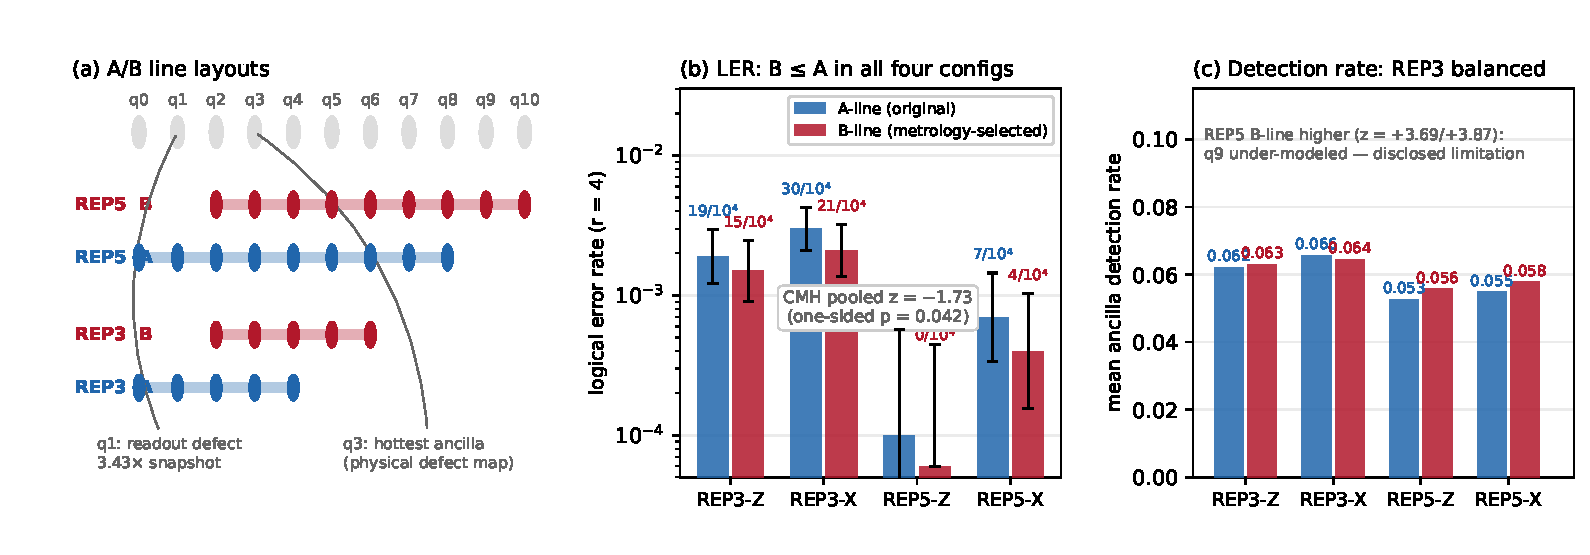
\includegraphics[width=\columnwidth]{figures/ap_f2_ab_result.pdf}
\caption{Active provenance: (a) A/B line layout with defect annotations;
  (b) logical error rates with Wilson CIs and the CMH pool;
  (c) per-detector event rates with the REP5 dissociation disclosed.}
\label{fig:ab}
\end{figure}

\section{Pre-registered device test of the injection-budget bound}
\label{app:injection}
%%-----------------------------------------------------------

We test Theorem~\ref{thm:spacetime} and Corollary~\ref{cor:stoch} on
ibm\_marrakesh (156-qubit Heron r2) with REP5 ($d{=}5$, $t{=}2$) and
REP3 ($d{=}3$, $t{=}1$) memories, both sectors, $R{=}4$ rounds.
The adversary injects Pauli faults at round~2 (Z-sector: physical $X$
gates; X-sector: basis-conjugated physical $X$ gates, H--$X$--H, realizing
$Z$-type faults on the $\lvert +_L \rangle$ memory; each injected fault is
thus implemented with native gates in both sectors). Layouts are the metrology-selected B-lines of
Appendix~\ref{app:activeprov}, fixed across all arms so that injection
is the only varying factor. Predictions, decision rules, seeds,
layouts, and circuit digests were pinned (SHA-256
\texttt{759169c2\dots c74653cd5}) \emph{before} submission; 312 arms
(180{,}000 shots) ran in four Sampler jobs
(\texttt{da8um21qtnsc73d0v3ug}, \texttt{da8um2ce74ec73aj4n3g},
\texttt{da8um31qtnsc73d0v400}, \texttt{da8um3ke74ec73aj4n50}); the full
noiseless pipeline was validated end-to-end (22/22 arms) before
submission. $\pi(k)$ entering the composed bounds is estimated from the
calibration-snapshot fault model ($\lambda_N{=}0.47$ faults/shot REP5,
$0.25$ REP3): $\pi(1..3)=0.375, 0.081, 0.012$ (REP5) and
$0.221, 0.027, 0.002$ (REP3). Scope: this campaign tests the
injection-budget bound and the calibration-to-model workflow on
repetition memories; it is not a measurement of BB-code hardware
performance, and no quantitative REP$\to$BB transfer is claimed.

\begin{table}[H]\centering\small
\caption{Deterministic worst-case injection arms (10{,}000 shots each).
``Bound'': Theorem~\ref{thm:spacetime}(c) with calibration $\pi$.}
\label{tab:injdet}
\begin{tabular}{@{}llrrrr@{}}
\toprule
arm & sector & failures & LER & bound & verdict \\\midrule
REP5 base & Z & 0 & 0.0000 & 0.012 & holds \\
REP5 base & X & 2 & 0.0002 & 0.012 & holds \\
REP5 $w{=}2$ worst & Z & 414 & 0.0414 & 0.375 & holds \\
REP5 $w{=}2$ worst & X & 506 & 0.0506 & 0.375 & holds \\
REP5 $w{=}3$ worst & Z & 9590 & 0.9590 & --- & sharp \\
REP5 $w{=}3$ worst & X & 9598 & 0.9598 & --- & sharp \\
REP3 base & Z & 14 & 0.0014 & 0.027 & holds \\
REP3 base & X & 28 & 0.0028 & 0.027 & holds \\
REP3 $w{=}1$ worst & Z & 276 & 0.0276 & 0.221 & holds \\
REP3 $w{=}1$ worst & X & 318 & 0.0318 & 0.221 & holds \\
REP3 $w{=}2$ worst & Z & 9292 & 0.9292 & --- & sharp \\
REP3 $w{=}2$ worst & X & 9240 & 0.9240 & --- & sharp \\\bottomrule
\end{tabular}
\end{table}

\begin{table}[H]\centering\small
\caption{Stochastic injection arms, REP5 (50 pinned variants $\times$ 200
shots per cell). Naive: $\delta_0+\Pr[\mathrm{Bin}\ge3]+\mathrm{tol}$;
composed: Corollary~\ref{cor:stoch} with calibration $\pi$.}
\label{tab:injstoch}
\begin{tabular}{@{}llrrrrl@{}}
\toprule
$p$ & sector & failures & LER & naive & composed & naive verdict \\\midrule
0.01 & Z & 1 & 0.0001 & 0.0020 & 0.016 & holds \\
0.01 & X & 2 & 0.0002 & 0.0020 & 0.016 & holds \\
0.05 & Z & 6 & 0.0006 & 0.0031 & 0.035 & holds \\
0.05 & X & 9 & 0.0009 & 0.0031 & 0.035 & holds \\
0.10 & Z & 211 & 0.0211 & 0.0101 & 0.070 & \textbf{falsified} \\
0.10 & X & 388 & 0.0388 & 0.0101 & 0.070 & \textbf{falsified} \\\bottomrule
\end{tabular}
\end{table}

Three findings. (i)~\emph{The distance cliff is real and sharp:}
weight-$t$ worst-case injections stay within the composed
correctability bound on both distances and both sectors, while
weight-$(t{+}1)$ injections collapse the memory at $92.4$--$96.0\%$
logical failure; the shortfall from $100\%$ is native-noise rescue of
order $\pi(1)$. (ii)~\emph{Injection amplifies native noise exactly as
the chain argument predicts:} the REP5 $w{=}2$ arms sit
$100$--$250\times$ above baseline but an order of magnitude inside the
composed bound --- the first quantitative measurement of
adversary--noise composition on a quantum memory.
(iii)~\emph{The independence-form stochastic bound
(Proposition~\ref{prop:stochastic}) is falsified on device} at
$p{=}0.10$ by $2.1\times$ (Z) and $3.8\times$ (X), while the
device-aware composed form holds on all six stochastic arms and all
eight bounded deterministic arms. The hardware data selects
Corollary~\ref{cor:stoch} over the independence form: a theory
refinement driven by device data, made possible only by pre-registering
the falsifiable version.

\paragraph{Security corollary.}
Combined with the REP5 detection-rate dissociation of
Appendix~\ref{app:activeprov} (placement moves the detection rate, not
the logical rate), these results imply that syndrome-level statistics
cannot certify memory integrity: a memory is certifiably
$(W,\eta)$-integrity-secure --- $\lambda_{\mathcal{M}}(W)\le\eta$ under
$\mathfrak{A}_1^{\mathrm{st}}(W)$ --- only via logical-level injection
probing of the kind reported here.

\subsection{Replication: second calibration cycle, second device,
distance~7}\label{app:injection-repl}

A pre-registered consolidation campaign (predictions, decision rules,
seeds, layouts, estimator, and digests pinned before submission, SHA-256
\texttt{cef236ce\dots de53aa1}) re-ran the test on
ibm\_marrakesh on a second calibration cycle (2026-09-06; 240{,}000
shots in four Sampler jobs \texttt{daelek5nj4cs73afaqpg},
\texttt{daelekd1ierc738mai50}, \texttt{daelel642tqs73auss4g},
\texttt{daeleljdd5gc73d8pcrg}), extended it to REP7 ($d{=}7$, $t{=}3$;
worst-case central strings $w{=}3$ and $w{=}4$), and replicated the REP5
deterministic arms on a second device, ibm\_fez (60{,}000 shots; jobs
\texttt{daelelt1ierc738mai7g}, \texttt{daelembdd5gc73d8pct0}). Layouts
were re-selected from the pinned 2026-09-06 snapshots by the
metrology rule of Appendix~\ref{app:activeprov} (the REP5 rule returned
the campaign-1 line); the stochastic masks are bit-identical to
campaign~1. The native-fault estimator is pinned explicitly,
$\lambda_N=\sum_{\mathrm{data}}\epsilon_{\mathrm{ro}}+
R\sum_{\mathrm{anc}}\epsilon_{\mathrm{ro}}$ with symmetric readout
$\epsilon_{\mathrm{ro}}$ (readout locations dominate the Heron-r2
spacetime budget; gate/idle terms are second order): $\lambda_N{=}0.088,
0.222, 0.347$ (REP3/5/7, marrakesh) and $0.453$ (REP5, fez) --- the
2026-09-06 marrakesh calibration is substantially cleaner than that of
2026-08-28 ($\lambda_N{=}0.25, 0.47$). Noiseless end-to-end validation
passed on all 42 checked arms before submission.

\begin{table}[H]\centering\small
\caption{Consolidation deterministic arms (10{,}000 shots each): REP7
extension (ibm\_marrakesh) and second-device REP5 replication
(ibm\_fez). ``Bound'': Theorem~\ref{thm:spacetime}(c) with the pinned
calibration $\pi$.}
\label{tab:injrepl}
\begin{tabular}{@{}lllrrrl@{}}
\toprule
device & arm & sector & failures & LER & bound & verdict \\\midrule
marrakesh & REP7 base & Z & 0 & 0.0000 & 0.0005 & holds \\
 & REP7 $w{=}3$ worst & Z & 568 & 0.0568 & 0.293 & holds \\
 & REP7 $w{=}4$ worst & Z & 9691 & 0.9691 & --- & sharp \\
 & REP7 base & X & 1 & 0.0001 & 0.0005 & holds \\
 & REP7 $w{=}3$ worst & X & 675 & 0.0675 & 0.293 & holds \\
 & REP7 $w{=}4$ worst & X & 9599 & 0.9599 & --- & sharp \\\midrule
fez & REP5 base & Z & 1 & 0.0001 & 0.011 & holds \\
 & REP5 $w{=}2$ worst & Z & 484 & 0.0484 & 0.364 & holds \\
 & REP5 $w{=}3$ worst & Z & 9768 & 0.9768 & --- & sharp \\
 & REP5 base & X & 6 & 0.0006 & 0.011 & holds \\
 & REP5 $w{=}2$ worst & X & 683 & 0.0683 & 0.364 & holds \\
 & REP5 $w{=}3$ worst & X & 9745 & 0.9745 & --- & sharp \\\bottomrule
\end{tabular}
\end{table}

Four findings. (i)~\emph{Full replication.} On the new calibration cycle
every campaign-1 verdict reproduces: all bounded deterministic arms sit
$4$--$8\times$ inside the composed bound on both distances and sectors
(REP3 $w{=}1$: $0.0102/0.0202$ vs bound $0.084$; REP5 $w{=}2$:
$0.0333/0.0436$ vs $0.199$), all weight-$(t{+}1)$ arms remain sharp
($0.898$--$0.974$), and all six stochastic cells track campaign~1 within
statistical noise (at $p{=}0.10$: $0.0202$ vs $0.0211$ Z; $0.0403$ vs
$0.0388$ X) --- including the falsification of the independence-form
bound, which replicates at $1.9\times$ (Z) and $3.6\times$ (X).
(ii)~\emph{The cliff has a third distance point.} REP7 behaves as
Theorem~\ref{thm:spacetime} demands: weight-$3$ worst-case injections
stay inside the bound ($0.057/0.068$ vs $0.293$) while weight-$4$
collapses the memory at $96.0$--$96.9\%$; the cliff is sharp at
$d{=}3,5,7$. (iii)~\emph{Cross-device.} The REP5 pattern reproduces on
ibm\_fez with its own pinned calibration ($\lambda_N{=}0.453$): bounds
hold at $5$--$7\times$ margin, sharpness at $97.5$--$97.7\%$.
(iv)~\emph{Mask-level composition.} With the cleaner calibration the
binomial-form composed bound tightens, and the X-sector $p{=}0.10$ cell
($0.0403$) exceeds it by $1.20\times$; the excess is entirely accounted
for by the realized pinned-mask ensemble --- the X masks contain two
weight-3 variants versus $0.43$ expected under $\mathrm{Bin}(5,0.1)$,
contributing $0.0375$ --- and conditioning the composed bound on the
realized masks (bound $0.067$) restores it: the composition law holds
mask-by-mask, not only in binomial expectation. Absolute LERs of bounded
arms drift down coherently with the cleaner calibration
($\lambda_N$: $0.47{\to}0.22$), while cliff arms drift slightly up (less
native-noise rescue of order $\pi(1)$), exactly as the model predicts.
The consolidation artifacts (\texttt{theory\_test\_consol/}) are archived
with the same digest discipline as campaign~1.

%%-----------------------------------------------------------
\section{Illustrative routing arithmetic}\label{app:routing}
\emph{Heuristic only; LFR underestimates diamond-norm error.}
$J=8$, $b=1$, $\Delta=0.05$: $p_\mathrm{hit}\le0.175$.
CZ at $p=5\times10^{-4}$: $(0.825)(0.905)=0.747$.
MS: $(0.825)(0.955)=0.788$.

\bibliographystyle{unsrtnat}
\bibliography{references}
\end{document}
